\documentclass{article}
\pdfpagewidth=8.5in
\pdfpageheight=11in

\usepackage{kr}

\usepackage{times}
\usepackage{soul}
\usepackage{url}
\usepackage[hidelinks]{hyperref}
\usepackage[utf8]{inputenc}
\usepackage[small]{caption}
\usepackage{graphicx}
\usepackage{amsmath}
\usepackage{amsthm}
\usepackage{booktabs}
\urlstyle{same}

\usepackage[backgroundcolor=lightgray]{todonotes}
\usepackage{listings}
\usepackage[linesnumbered,ruled,vlined]{algorithm2e}
\usepackage[capitalize,noabbrev]{cleveref}
\usepackage{microtype}
\usepackage{mathtools}
\usepackage{forest}
\usepackage{siunitx}
\usepackage{amsfonts}
\usepackage{pifont}
\usepackage[inline]{enumitem}

\usetikzlibrary{arrows.meta}

\newtheorem{theorem}{Theorem}
\newtheorem{fact}{Fact}
\theoremstyle{definition}
\newtheorem{definition}{Definition}
\newtheorem{example}{Example}

\pdfinfo{
/TemplateVersion (KR.2022.0, KR.2023.0, KR.2024.0)
}

\forestset{
  sn edges/.style={for tree={edge={-Latex}}}
}

\lstset{breaklines=true}
\lstset{language=C++,
        basicstyle=\ttfamily,
        stringstyle=\color{red},
        commentstyle=\color{green},
        breaklines=true,
        showstringspaces=false}

\crefname{line}{line}{lines}

\crefalias{enumi}{type}
\crefname{type}{Type}{Types}
\creflabelformat{type}{#2\textup{#1}#3}

\crefalias{clause}{equation}
\crefname{clause}{Clause}{Clauses}
\creflabelformat{clause}{#2\textup{(#1)}#3}

\crefalias{formula}{equation}
\crefname{formula}{Formula}{Formulas}
\creflabelformat{formula}{#2\textup{(#1)}#3}

\DeclareMathOperator{\CR}{CR}
\DeclareMathOperator{\DR}{DR}
\DeclareMathOperator{\Reff}{Ref}

\DeclareMathOperator{\Doms}{Doms}
\DeclareMathOperator*{\argmin}{argmin} % TODO: soon to be removed

\newcommand{\cmark}{\ding{51}}
\newcommand{\xmark}{\ding{55}}

\newcommand{\expr}{\mathtt{expr}}
\newcommand{\Ctwo}{$\mathsf{C}^{2}$}
\newcommand{\FO}{$\mathsf{FO}$}
\newcommand{\UFO}{$\mathsf{UFO}^{2} + \mathsf{EQ}$}

\newcommand{\Cranetwo}{\textsc{Crane2}}
\newcommand{\Cranebfs}{\textsc{Crane2-BFS}}
\newcommand{\Cranegreedy}{\textsc{Crane2-Greedy}}

\SetKwFunction{CompileWithBaseCases}{CompileWithBaseCases}
\SetKwFunction{Crane}{Compile}
\SetKwFunction{Propagate}{Propagate}
\SetKwFunction{FindBaseCases}{FindBaseCases}
\SetKwFunction{Simplify}{Simplify}

\title{Towards Practical First-Order Model Counting}

\author{%
  Ananth K. Kidambi$^1$\footnote{The first and second authors contributed equally and were affiliated with the National University of Singapore during the completion of this work.}\and
Guramrit Singh$^1$\and
Paulius Dilkas$^2$\and
Kuldeep S. Meel$^3$ \\
\affiliations
$^1$Indian Institute of Technology Bombay, Mumbai, India\\
$^2$National University of Singapore, Singapore, Singapore\\
$^3$University of Toronto, Toronto, Canada\\
\emails
\{210051002, 210050061\}@iitb.ac.in,
paulius.dilkas@nus.edu.sg,
meel@cs.toronto.edu
}

\begin{document}

\maketitle

\begin{abstract}
  TODO: at most 200 words
\end{abstract}

\section{Introduction (TODO)}

\todo[inline,caption={}]{
  \begin{itemize}
    \item 9 pages!!!
    \item Add some papers mentioned in:
          \begin{itemize}
            \item very recent work
            \item my previous paper, including:
                  \begin{itemize}
                    \item other liftable fragments
                    \item some more theory papers, e.g., LICS 2018
                  \end{itemize}
          \end{itemize}
  \end{itemize}
}

\paragraph{Papers To Cite}
\begin{itemize}
  \item overviews
        \begin{itemize}
          \item lifted probabilistic inference~\cite{DBLP:conf/ecai/Kersting12}
          \item recent overview paper~\cite{DBLP:conf/ijcai/Kuzelka23}
        \end{itemize}
  \item Alternative definition~\cite{DBLP:journals/cacm/GogateD16}
  \item relevant theoretical work~\cite{DBLP:conf/aaai/MalhotraS22}
  \item original domain recursion~\cite{DBLP:conf/nips/Broeck11}
  \item algorithms
        \begin{itemize}
          \item \textsc{ForcLift}~\cite{DBLP:conf/ijcai/BroeckTMDR11}
          \item \textsc{Crane}~\cite{DBLP:conf/kr/DilkasB23}
          \item \textsc{FastWFOMC}~\cite{DBLP:conf/uai/BremenK21}
          \item \textsc{L2C}~\cite{DBLP:conf/kr/KazemiP16} (similarly to us
                compiles to C++ code, but (probably) doesn't work on as many
                formulas)
          \item approximate~\cite{DBLP:conf/ijcai/BremenK20}
          \item for Markov logic networks~\cite{DBLP:journals/ml/RichardsonD06}
                \begin{itemize}
                  \item \textsc{Magician}~\cite{DBLP:conf/aaai/VenugopalSG15}
                  \item \textsc{Tuffy}~\cite{DBLP:journals/pvldb/NiuRDS11}
                  \item \textsc{Alchemy}~\cite{DBLP:journals/cacm/GogateD16}
                        (same as the alternative definition)
                \end{itemize}
        \end{itemize}
  \item complexity
        \begin{itemize}
          \item liftability~\cite{DBLP:conf/starai/JaegerB12}
          \item hardness for three variables~\cite{DBLP:conf/pods/BeameBGS15}
          \item liftable fragments
                \begin{itemize}
                  \item \Ctwo~\cite{DBLP:journals/jair/Kuzelka21}
                  \item tree axioms~\cite{DBLP:journals/ai/BremenK23}
                  \item linear order axioms~\cite{DBLP:conf/aaai/TothK23}
                  \item some liftable fragments~\cite{DBLP:conf/nips/KazemiKBP16}
                \end{itemize}
        \end{itemize}
  \item applications
        \begin{itemize}
          \item extensions to
                sampling~\cite{DBLP:conf/aaai/WangB0K22,DBLP:conf/lics/WangP0K23}
          \item discovery of combinatorial
                sequences~\cite{DBLP:conf/ijcai/SvatosJT0K23}
          \item conjecturing recurrence
                relations~\cite{DBLP:conf/ilp/BarvinekB0ZK21}
          \item probabilistic logic
                programming~\cite{DBLP:journals/ijar/RiguzziBZCL17} (WFOMC was
                shown to be supreme)
          \item probabilistic databases~\cite{DBLP:journals/debu/GribkoffSB14}
        \end{itemize}
  \item lifted inference elsewhere
        \begin{itemize}
          \item constraint satisfaction~\cite{DBLP:journals/jair/TotisDRK23}
          \item answer set programming~\cite{DBLP:journals/ijar/AzzoliniR23}
        \end{itemize}
\end{itemize}

\begin{figure*}[t]
  \centering
  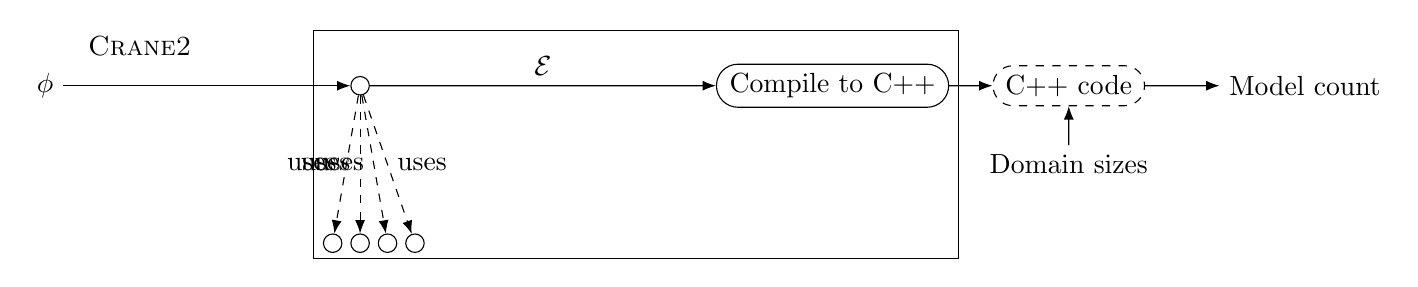
\begin{tikzpicture}
    \node at (-1, 0) (formula) {$\phi$};
    \node[draw,rounded rectangle] at (3, 0) (alg1) {\CompileWithBaseCases};
    \node[draw,rounded rectangle] at (9, 0) (compilation) {Compile to C++};

    \node[draw,rounded rectangle,dashed] at (12, 0) (cpp) {C++ code};
    \node at (12, -1) (sizes) {Domain sizes};

    \node at (15, 0) (count) {Model count};

    \node[draw,rounded rectangle] at (3, -2) (alg2) {\FindBaseCases};
    \node[draw,rounded rectangle,left = 0.1cm of alg2] (crane) {\Crane};
    \node[draw,rounded rectangle,right = 0.1cm of alg2] (alg3) {\Propagate};
    \node[draw,rounded rectangle,right = 0.1cm of alg3] (simplify) {\Simplify};

    \node[draw,fit={(alg1) (compilation) (crane) (alg2) (alg3)},inner ysep=7pt,yshift=5pt] {};
    \node at (0.2, 0.5) {\Cranetwo};

    \draw[-Latex] (formula) -- (alg1);
    \draw[-Latex] (alg1) -- node[above] {$\mathcal{E}$} (compilation);
    \draw[-Latex] (compilation) -- (cpp);
    \draw[-Latex] (sizes) -- (cpp);
    \draw[-Latex] (cpp) -- (count);

    \draw[-Latex,dashed] (alg1) -- node[midway,left] {uses} (crane);
    \draw[-Latex,dashed] (alg1) -- node[midway,left] {uses} (alg2);
    \draw[-Latex,dashed] (alg1) -- node[midway,left] {uses} (alg3);
    \draw[-Latex,dashed] (alg1) -- node[midway,right] {uses} (simplify);
  \end{tikzpicture}
  \caption[]{The outline of using \Cranetwo{} to compute the model count of a
    formula $\phi$. The formula is compiled into a set of equations
    $\mathcal{E}$ that are then compiled to a C++ program. This program can then
    be run with different command line arguments to compute the model count of
    $\phi$ for various domain sizes. \CompileWithBaseCases makes use
    of: \begin{enumerate*}[label=(\roman*)]
      \item the knowledge compilation algorithm of \textsc{Crane} (denoted by \Crane),
      \item a procedure for identifying a sufficient set of base cases (denoted by \FindBaseCases),
      \item a procedure for constructing a formula that corresponds to a given base case (denoted by \Propagate), and
      \item algebraic simplification techniques (denoted by \Simplify).
    \end{enumerate*}
  }\label{fig:overview}
\end{figure*}

\todo[inline]{By pointing to the outline in \cref{fig:overview}, make forward
  references to the sections of the paper.}

\paragraph{Contributions}
\begin{itemize}
  \item Completing the definitions of recursive functions by:
  \begin{itemize}
    \item identifying a sufficient set of base cases (\cref{sec:identifying})
    \item constructing formulas that correspond to these base cases
          (\cref{sec:simplifying})
    \item and recursing on these subproblems
  \end{itemize}
  \item Compiling these function definitions into a C++ program that can be
        executed independently for any domain size values \cref{sec:cpp}
        \begin{itemize}
          \item including support for infinite precision arithmetic via GNU
                Multiple Precision Arithmetic Library
        \end{itemize}
  \item Experiments comparing \Cranetwo{} with the main alternative approach
        demonstrate the ability of \Cranetwo{} to scale to domain sizes\dots
\end{itemize}

\Cref{sec:identifying,sec:cpp} deal with algebraic constructs whereas
\cref{sec:simplifying} deals with logic.

\section{Preliminaries (TODO)}

\Cref{sec:logic} introduces the fundamental ideas of first-order logic and
WFOMC, and discusses the different logics used in the latter.\@
\Cref{sec:algebra} introduces the terminology we use to describe the output of
the original \textsc{Crane} algorithm~\cite{DBLP:conf/kr/DilkasB23}, i.e.,
functions and equations that define them.

We write $\mathbb{N}_{0}$ for the set of non-negative integers. In the context
of both algebra and logic, we write $C[x \mapsto y]$ for $C$ with all
occurrences of $x$ replaced with $y$.

\subsection{Logic (TODO)}\label{sec:logic}

\todo[inline]{Clarify the differences between the input format and the internal
  format}

\paragraph{The \FO{} Logic (After Skolemization and in a special (prenex, CNF)
  form)}
\begin{itemize}
  \item Although existential quantifiers are supported, here we describe the
        format used internally. During preprocessing, all existential
        quantifiers are eliminated using
        Skolemization~\cite{DBLP:conf/kr/BroeckMD14}, and the formula is
        rewritten into a conjunction of clauses, each of which is in
        \emph{prenex normal form}~\cite{hinman2018fundamentals}.
  \item In the spirit of keeping sorts implicit, we always assume formulas `type
        check' with respect to sorts. For example, if $P(x)$, $P(y)$, and
        $x \ne c$ are all part of the formula (for some predicate $P$, variables
        $x$ and $y$, and constant $c$), then $x$, $y$, and $c$ all have the same
        sort.
  \item A \emph{formula} is a conjunction of clauses.
  \item A \emph{clause} is of the form $\forall x_{1} \in \Delta_{1}\text{.
        }\forall x_{2} \in \Delta_{2}\dots\text{
        }\forall x_{n} \in \Delta_{n}\text{. }\phi(x_{1}, x_{2}, \dots, x_{n})$,
        where $\phi$ is a disjunction of literals that only contain variables
        $x_{1}, \dots, x_{n}$ (and any constants).
  \item We say that a clause is a \emph{(positive) unit clause} if:
        \begin{itemize}
          \item there is only one literal with a predicate, and
          \item it is a positive literal.
        \end{itemize}
  \item A \emph{literal} is either an atom (i.e., a \emph{positive} literal) or
        its negation (i.e., a \emph{negative} literal).
  \item An \emph{atom} is either:
  \begin{itemize}
    \item $P(t_{1}, \dots, t_{m})$ for some predicate $P/m$ and terms
          $t_{1}, \dots, t_{m}$ or
    \item $x=y$ for some terms $x$ and $y$
  \end{itemize}
  \item An atom is \emph{ground} if it contains no variables (i.e., only
        constants).
  \item The \emph{arity} of a predicate is the number of arguments it takes,
        i.e., $m$ in the case of predicate $P$.
  \item When we want to denote a predicate together with its arity, we write
        $P/m$.
  \item A \emph{term} is either a variable or a constant.
  \item Throughout the paper, we use set-theoretic notation, interpreting a
        formula as a set of clauses and a clause as a set of literals. Moreover,
        for readability, clauses written on separate lines are implicitly
        conjoined.
\end{itemize}

\begin{definition}[Model]\label{def:model}
  Let $\phi$ be a formula in \FO{}. For every predicate $p/n$ in $\phi$, let
  ${(\Delta_{i}^{p})}_{i=1}^{n}$ be a list of the corresponding domains (not
  necessarily distinct). Let $\sigma$ be a map from the domains of $\phi$ to
  their interpretations as sets such that:
  \begin{itemize}
    \item the sets are pairwise disjoint, and
    \item the constants in $\phi$ are included in the corresponding domains.
  \end{itemize}
  Then a \emph{structure} of $\phi$ (with respect to $\sigma$) is a set $M$ of
  ground literals defined by adding either $p(\mathbf{t})$ or
  $\neg p(\mathbf{t})$ for every predicate $p/n$ in $\phi$ and $n$-tuple
  $\mathbf{t} \in \prod_{i=1}^{n} \sigma(\Delta_{i}^{p})$. A structure is a
  \emph{model} if it satisfies $\phi$ (see Appendix~A of~Dilkas and
  Belle~\shortcite{DBLP:journals/corr/abs-2306-04189} for more details).
\end{definition}

\begin{definition}[WFOMC]
  Continuing from \cref{def:model}, for every predicate $p/n$ in $\phi$, let
  $w^{+}(p), w^{-}(p) \in \mathbb{R}$ be its (positive and negative)
  \emph{weights}. Unless explicitly specified otherwise, we assume weights to be
  equal to one. The \emph{(symmetric) weighted first-order model count} (WFOMC)
  of $\phi$ (with respect to $\sigma$, $w^{+}$, and $w^{-}$) is the quantity
  \[
    \sum_{M \models \phi} \prod_{p(\mathbf{t}) \in M} w^{+}(p) \prod_{\neg p(\mathbf{t}) \in M} w^{-}(p),
  \]
  where the sum is over all models of $\phi$.
\end{definition}

\begin{table*}
  \centering
  \begin{tabular}{llclll}
    \toprule
    Logic & Sorts & Constants & Variables & Quantifiers & Additional atoms\\
    \midrule
    \FO & one or more & \cmark & unlimited & $\forall$, $\exists$ & $x = y$\\
    \Ctwo & one & \xmark & two & $\forall$, $\exists$, $\exists^{= k}$, $\exists^{\le k}$, $\exists^{\ge k}$ & ---\\
    \UFO & one & \xmark & two & $\forall$ & $|P| = m$\\
    \bottomrule
  \end{tabular}
  \caption[]{A comparison of the three logics used in WFOMC in terms of:
    \begin{enumerate*}[label=(\roman*)]
      \item the number of sorts,
      \item support for constants,
      \item the maximum number of variables,
      \item allowed quantifiers, and
      \item supported atoms in addition to those of the form $P(\mathbf{t})$ for some predicate $P/n$ and $n$-tuple of terms $\mathbf{t}$.
    \end{enumerate*}
    Here:
    \begin{enumerate*}[label=(\roman*)]
      \item $k, m \in \mathbb{N}_{0}$, the latter of which can depend on the domain size,
      \item $P$ is a predicate, and
      \item $x$ and $y$ are terms.
    \end{enumerate*}
  }\label{tbl:logics}
\end{table*}

\paragraph{Three Types of Logics}
\begin{itemize}
  \item See \cref{tbl:logics} for a detailed comparison. The notation introduced
        in the table is standard for \Ctwo{}, new for \UFO{}, and redefined to
        be more specific for \FO{}.
  \item All three logics are function-free.
  \item Domains are always assumed to be finite.
  \item In many-sorted logic, each term is assigned to a \emph{sort}, and each
        predicate $p/n$ is assigned to a sequence of $n$ sorts. Each sort has
        its corresponding domain. In the input formula, all domains are assumed
        to be pairwise disjoint Most of these assignments are typically left
        implicit and can be reconstructed from the quantifiers. For instance,
        $\forall x,y \in \Delta\text{. }P(x, y)$ implies that variables $x$ and
        $y$ have the same sort. On the other hand, $\forall x \in \Delta\text{.
        }\forall y \in \Gamma\text{. } P(x, y)$ implies that $x$ and $y$ have
        different sorts, and it would be improper to have $x = y$ as part of a
        formula.
  \item
        \begin{itemize}
          \item \FO{} is used as the input format for
                \textsc{ForcLift}\footnote{\url{https://github.com/UCLA-StarAI/Forclift}}~\cite{DBLP:conf/ijcai/BroeckTMDR11}
                and its extensions
                \textsc{Crane}\footnote{\url{https://doi.org/10.5281/zenodo.8004077}}~\cite{DBLP:conf/kr/DilkasB23}
                and \Cranetwo{}.
          \item \Ctwo{} is discussed in the literature on
                \textsc{FastWFOMC}~\cite{DBLP:conf/uai/BremenK21} and related
                methods~\cite{DBLP:journals/jair/Kuzelka21,DBLP:conf/aaai/MalhotraS22}
          \item \UFO{} is the input format supported by a version of
                \textsc{FastWFOMC} obtained directly from the authors. Note that
                the publicly available
                version\footnote{\url{https://comp.nus.edu.sg/~tvanbr/software/fastwfomc.tar.gz}}
                does not support any cardinality constraints.
        \end{itemize}
  \item Note that, in the case of \textsc{ForcLift} and its extensions, support
        for a formula as valid input does not imply that the algorithm will be
        able to compile the formula into a circuit or graph suitable for lifted
        model counting. However, it is known that \textsc{ForcLift} compilation
        is guaranteed to succeed on any \FO{} formula without constants and with
        at most two variables~\cite{DBLP:conf/nips/Broeck11}.
\end{itemize}

\begin{example}\label{example:functions}
  Functions
  \begin{itemize}
    \item In \Ctwo: $\forall x \in \Delta\text{.
          }\exists^{=1} y \in \Delta\text{. }P(x, y)$
    \item In \UFO:
          \begin{gather*}
            \forall x, y \in \Delta\text{. }S(x) \lor \neg P(x, y)\\
            |P| = |\Delta|
          \end{gather*}
    \item In \FO:
          \begin{gather*}
            \forall x \in \Delta\text{. }\exists y \in \Delta\text{. }P(x, y)\\
            \forall x, y, z \in \Delta\text{. }P(x, y) \land P(x, z) \Rightarrow y = z
          \end{gather*}
  \end{itemize}
\end{example}

\subsection{Algebra}\label{sec:algebra}

We write $\expr{}$ for an arbitrary algebraic expression. Note that some terms
have different meanings in the context of algebra as compared to logic. Here, a
\emph{constant} is a non-negative integer. Similarly, a \emph{variable} is
either a parameter of a function or a variable introduced by a summation, e.g.,
$i$ in $\sum_{i=1}^{n} \expr$. A (function) \emph{signature} is
$f(x_{1}, \dots, x_{n})$ (written $f(\mathbf{x})$ for short), where $f$ is an
$n$-ary function, and each $x_{i}$ is a variable. An \emph{equation} is
$f(\mathbf{x}) = \expr{}$, where $f(\mathbf{x})$ is a signature.

\begin{definition}
  Let $f$ be a function with signature $f(\mathbf{x})$. Then a \emph{base case}
  of $f$ is a function call $f(\mathbf{y})$ such that either $y_{i} = x_{i}$ or
  $y_{i} \in \mathbb{N}_{0}$ for all $i$, and the latter case applies at least
  once.
\end{definition}

\section{Completing the Definitions of Recursive Functions}\label{sec:main}

\begin{algorithm}[t]
  \caption{\protect\CompileWithBaseCases{$\phi$}}\label{alg:main}
  \KwIn{formula $\phi$}
  \KwOut{set $\mathcal{E}$ of equations}
  $(\mathcal{E}, \mathcal{F}, \mathcal{D}) \gets \Crane{$\phi$}$\;\label{line:first}
  $\mathcal{E} \gets \Simplify{$\mathcal{E}$}$\;\label{line:second}
  \ForEach{base case $f(\mathbf{x}) \in \FindBaseCases{$\mathcal{E}$}$}{
    $\psi \gets \mathcal{F}(f)$\;
    \ForEach{$i$ such that $x_{i} \in \mathbb{N}_{0}$}{
      $\psi \gets \Propagate{$\psi$, $\mathcal{D}(f, i)$, $x_i$}$\;
    }
    $\mathcal{E} \gets \mathcal{E} \cup \CompileWithBaseCases{$\psi$}$\;
  }
\end{algorithm}

\Cref{alg:main} outlines our overall approach for compiling a formula into a set
of equation that include the required base cases. In short, we first use the
knowledge compilation algorithm of the original
\textsc{Crane}~\cite{DBLP:conf/kr/DilkasB23} to compile the formula into:
\begin{enumerate*}[label=(\roman*)]
  \item set $\mathcal{E}$ of equations,
  \item map $\mathcal{F}$ from function names to formulas, and
  \item map $\mathcal{D}$ from function names and argument indices to domains.
\end{enumerate*}
After some algebraic simplification, $\mathcal{E}$ is passed to the
\FindBaseCases procedure (described in \cref{sec:identifying}) that returns a
set of base cases that we need to find solutions for. For each base case
$f(\mathbf{x})$, we identify the formula associated with $f$ and simplify it
using the \Propagate procedure (described in \cref{sec:simplifying}). The
algorithm then recurses on these simplified formulas and adds the resulting base
case equations to $\mathcal{E}$. \Cref{example:overall} explains \cref{alg:main}
in more detail.

\begin{example}\label{example:overall}
  Let us consider the following formula (previously examined by Dilkas and
  Belle~\shortcite{DBLP:conf/kr/DilkasB23}) that defines predicate $P$ to be a
  bijection between two sets $\Gamma$ and $\Delta$:
  \[
    \begin{gathered}
      \forall x \in \Gamma\text{. }\exists y \in \Delta\text{. }P(x, y)\\
      \forall y \in \Delta\text{. }\exists x \in \Gamma\text{. }P(x, y)\\
      \forall x \in \Gamma\text{. }\forall y, z \in \Delta\text{. }P(x, y) \land P(x, z) \Rightarrow y = z\\
      \forall x, z \in \Gamma\text{. }\forall y \in \Delta\text{. }P(x, y) \land P(z, y) \Rightarrow x = z.
    \end{gathered}
  \]
  In particular, we examine the first solution that \Cranebfs{} returns for this
  formula.

  After \cref{line:first,line:second}, we have
  \begin{align*}
    \mathcal{E} &= \left\{\,\begin{aligned}f(m, n) &= \sum_{l=0}^{n} \binom{n}{l}{(-1)}^{n-l}g(l, m),\\ g(l, m) &= g(l-1, m) + mg(l-1, m-1)\end{aligned}\,\right\};\\
    \mathcal{D} &= \{\, (f, 1) \mapsto \Gamma, (f, 2) \mapsto \Delta, (g, 1) \mapsto \Delta^{\top}, (g, 2) \mapsto \Gamma \,\},
  \end{align*}
  where $\Delta^{\top}$ is a new domain introduced by \Crane. Then
  \FindBaseCases identifies two base cases: $g(0, m)$ and $g(l, 0)$. In both
  cases, \CompileWithBaseCases recurses on the formula $\mathcal{F}(g)$
  simplified by assuming that one of the domains is empty. In the first case, we
  recurse on the formula $\forall x \in \Gamma\text{. }S(x) \lor \neg S(x)$,
  where $S$ is a predicate introduced by Skolemization with weights
  $w^{+}(S) = 1$ and $w^{-}(S) = -1$. Hence, we get the base case
  $g(0, m) = 0^{m}$. In the case of $g(l, 0)$, \Propagate{$\psi$, $\Gamma$, $0$}
  returns an empty formula, giving us $g(l, 0) = 1$.
\end{example}


Note that these base cases overlap when $l = m = 0$ but are consistent with each
other since $0^{0} = 1$. More generally, let $\phi$ be a formula with two
domains $\Gamma$ and $\Delta$, and let $n, m \in \mathbb{N}_{0}$. Then the model
count of \Propagate{$\phi$, $\Delta$, $n$} assuming $|\Gamma| = m$ is the same
as the model count of \Propagate{$\phi$, $\Gamma$, $m$} assuming $|\Delta| = n$.

\todo[inline]{Can I turn the above into a theorem?}

Finally, we note that the \Simplify procedure plays a crucial role in
simplifying a common algebraic pattern $\sum_{m=0}^{n}[a \le m \le b] f(m)$.
Here:
\begin{enumerate*}[label=(\roman*)]
  \item $n$ is a variable,
  \item $a, b \in \mathbb{N}_{0}$ are constants,
  \item $f$ is an expression that may depend on $m$, and
  \item $[a \le m \le b] =
  \begin{cases}
    1 & \text{if $a \le m \le b$} \\
    0 & \text{otherwise}
  \end{cases}$ is the Iverson bracket.
\end{enumerate*}
\Simplify transforms this pattern into
$f(a) + f(a+1) + \cdots + f(\min\{\, n, b \,\})$. For instance, in the case of
\cref{example:overall}, \Simplify transforms
$g(l, m) = \sum_{k=0}^{m}[0 \le k \le 1]\binom{m}{k}g(l-1, m-k)$ into the
simpler form above.

\todo[inline]{A concluding sentence that introduces the remaining subsections?}

\subsection{Identifying a Sufficient Set of Base Cases}\label{sec:identifying}

\begin{algorithm}[t]
  \caption{\protect\FindBaseCases{$\mathcal{E}$}}\label{alg1}
  \KwIn{set $\mathcal{E}$ of equations}
  \KwOut{set $\mathcal{B}$ of base cases}

  $\mathcal{B} \gets \emptyset$\;
  \ForEach{equation $(f(\mathbf{x}) = \expr{}) \in \mathcal{E}$}{
    \ForEach{function call $f(\mathbf{y}) \in \expr{}$}{\label{line:functioncall}
      \ForEach{$y_{i} \in \mathbf{y}$} {
        \uIf{$y_{i} \in \mathbb{N}_{0}$}{
          $\mathcal{B} \gets \mathcal{B} \cup \{\, f(\mathbf{x})[x_{i} \mapsto y_{i}] \,\}$\;
        }
        \ElseIf{$y_{i} = x_{i} - c_{i}$ for some $c_{i} \in \mathbb{N}_{0}$}{
          \For{$j \gets 0$ \KwTo $c_{i} - 1$}{\label{line:lim}
            $\mathcal{B} \gets \mathcal{B} \cup \{\, f(\mathbf{x})[x_{i} \mapsto j] \,\}$\;\label{line:insert}
          }
        }
      }
    }
  }
\end{algorithm}

\Cref{alg1} summarises the implementation of \FindBaseCases. For each recursive
call from a function $f$ to itself, we consider two types of arguments:
\begin{enumerate*}[label=(\roman*)]
  \item constants and
  \item arguments of the form $x_{i} - c_{i}$, where $c_{i} \in \mathbb{N}_{0}$
  is a constant, and $x_{i}$ is the $i$-th argument of the signature of $f$.
\end{enumerate*}
In the former case, we consider a base case specifically for that constant. In
the latter case, we consider a base case for constants from zero up to (but not
including) $c_{i}$. \Cref{thm:halting} below motivates this approach.

\begin{example}
  Consider the recursive function $g$ from \cref{example:overall}.
  \FindBaseCases{$\mathcal{E}$} iterates over two function calls: $g(l-1, m)$
  and $g(l-1, m-1)$. The former produces the base case $g(0, m)$, while the
  latter produces both $g(0, m)$ and $g(l, 0)$.
\end{example}

\todo[inline]{Prove (lots of notes, handwritten and elsewhere)}

\begin{theorem}[Halting]\label{thm:halting}
  Let us assume the following about the input set of equations $\mathcal{E}$:
  \begin{enumerate}
    \item Each function $f$ has exactly one equation with $f$ on the left-hand
          side.\@ We call this equation the \emph{definition} of $f$.
    \item There exists a topological ordering of all functions ${(f_{i})}_{i}$
          such that the definition of $f_{i}$ does not contain function calls to
          $f_{j}$ with $j > i$.\footnote{This condition excludes the possibility
          of mutual recursion and similar cyclic scenarios and is akin to
          stratified logic programs~\cite{DBLP:books/sp/Lloyd87}.}
    \item For every equation $(f(\mathbf{x}) = \expr) \in \mathcal{E}$, every
          recursive function call $f(\mathbf{y}) \in \expr$ satisfies the
          following:
          \begin{itemize}
            \item each $y_{i}$ is either $x_{i} - c_{i}$ or $c_{i}$ for some
                  constant $c_{i} \in \mathbb{N}_{0}$;
            \item there exists $i$ such that $y_{i} = x_{i} - c_{i}$ for some
                  $c_{i} > 0$.
          \end{itemize}
  \end{enumerate}
  Then the set of base cases $\mathcal{B}$ returned by
  \FindBaseCases{$\mathcal{E}$} is \emph{sufficient} for $\mathcal{E}$ in the
  following sense. The evaluation of any function call with non-negative
  arguments halts as long as the evaluation of base cases is prioritised over
  the corresponding recursive definitions.\footnote{Recall that, as previously
    discussed, the order in which base cases are considered is immaterial.}
\end{theorem}

\subsection{Propagating Domain Size Assumptions}\label{sec:simplifying}

\begin{algorithm}[t]
  \caption{\protect\Propagate{$\phi$, $\Delta$, $n$}}\label{alg2}
  \KwIn{formula $\phi$, domain $\Delta$, $n \in \mathbb{N}_{0}$}
  \KwOut{formula $\phi'$}
  $\phi' \gets \emptyset$\;
  \uIf{$n = 0$}{
    \ForEach{clause $C \in \phi$}{
      \lIf{$\Delta \not\in \Doms(C)$}{$\phi' \gets \phi' \cup \{\, C \,\}$}
      \Else{
        $C' \gets \{\, l \in C \mid \Delta \not\in \Doms(l) \,\}$\;
        \If{$C' \ne \emptyset$}{
          $l \gets \text{an arbitrary literal in } C'$\;\label{line:smoothing1}
          $\phi' \gets \phi' \cup \{\, C' \cup \{\, \neg l \,\} \,\} $\;\label{line:smoothing2}
        }
      }
    }
  }
  \Else{
    $D \gets \text{a set of $n$ new constants in $\Delta$}$\;
    \ForEach{clause $C \in \phi$}{
      ${(x_{i})}_{i=1}^{m} \gets \text{the variables in $C$ with domain $\Delta$}$\;
      \lIf{$m = 0$}{$\phi' \gets \phi' \cup \{\, C \,\}$}
      \Else{
        $\phi' \gets \phi' \cup \{\, C[x_{1} \mapsto c_{1}, \dots, x_{m} \mapsto c_{m}] \mid {(c_{i})}_{i=1}^{m} \in D^{m} \,\}$\;
      }
    }
  }
\end{algorithm}

\Propagate (\cref{alg2}) modifies formula $\phi$ with the assumption that domain
$\Delta$ has size $n \in \mathbb{N}_{0}$. In the case of $n=0$, many clauses
become vacuously satisfied and can be removed. In the case of
$n > 0$\footnote{None of the formulas considered in this work had $n > 1$.}, we
perform partial grounding, using constants to replace all variables quantified
over $\Delta$. \Cref{alg2} considers these two cases separately. For a literal
or a clause $C$, we write $\Doms(C)$ to denote the set of corresponding domains.

In the case of $n = 0$, consider three types of clauses:
\begin{enumerate*}[label=(\roman*)]
  \item those that do not mention $\Delta$,\label{type1}
  \item those in which every literal contains variables quantified over
  $\Delta$, and\label{type2}
  \item those that have some literals with variables quantified over $\Delta$
  and some without.\label{type3}
\end{enumerate*}
\Cref{type1} clauses are transferred to the new formula $\phi'$ unchanged. For
\cref{type2} clauses, $C' = \emptyset$, so these clauses are filtered out. One
might think that the same should be done with \cref{type3} clauses, however,
\cref{line:smoothing1,line:smoothing2} perform a new kind of smoothing, the
explanation of which we defer to \cref{sec:smoothingbase}.

In the case of $n>0$, we introduce $n$ new constants. Consider an arbitrary
clause $C \in \phi$ and let $m \in \mathbb{N}_{0}$ be the number of variables in
$C$ quantified over $\Delta$. If $m=0$, then, similarly to the previous case, we
add $C$ directly to $\phi'$. Otherwise, we add a clause to $\phi'$ with every
possible way of replacing the $m$ variables in $C$ with some combination of the
$n$ new constants.

\begin{example}
  Let us consider the clause $C \equiv \forall x \in \Gamma\text{.
  }\forall y, z \in \Delta\text{. } \neg P(x, y) \lor \neg P(x, z) \lor y=z$.
  Then
  $\Doms(C) = \Doms(\neg P(x, y)) = \Doms(\neg P(x, z)) = \{\, \Gamma, \Delta \,\}$,
  and $\Doms(y=z) = \{\, \Delta \,\}$. A call to \Propagate{$\{\, C \,\}$,
    $\Delta$, $3$} would produce the following formula with nine clauses:
  \begin{align*}
    \forall x \in \Gamma\text{. }\neg P(x, c_{1}) \lor& \neg P(x, c_{1}) \lor c_{1}=c_{1}\\
    \forall x \in \Gamma\text{. }\neg P(x, c_{1}) \lor& \neg P(x, c_{2}) \lor c_{1}=c_{2}\\
    \vdots&\\
    \forall x \in \Gamma\text{. }\neg P(x, c_{3}) \lor& \neg P(x, c_{3}) \lor c_{3}=c_{3},\\
  \end{align*}
  where $c_{1}$, $c_{2}$, and $c_{3}$ are the new constants.
\end{example}

\section{Smoothing (TODO)}

Goal of smoothing: whenever rules such as unit propagation or
inclusion-exclusion (maybe just these two?) eliminate the consideration of some
ground atoms, smoothing nodes should be inserted `at the same level' so that
these ground atoms are still considered when counting. Note that conjunction
nodes are irrelevant here because multiplication is associative. `At the same
level' means that, e.g., if some ground atoms were eliminated from consideration
before/after performing independent partial grounding, then the smoothing node
should also appear before/after the independent partial grounding node.

\todo[inline,caption={}]{
\begin{itemize}
  \item Cite something when introducing the idea of smoothing. Maybe both
        propositional and first-order sources.
  \item Can I prove that the additions to smoothing outlined in the rest of this
        section `do the right thing'?
\end{itemize}
}

\subsection{Smoothing for Base Cases (TODO)}\label{sec:smoothingbase}

\todo[inline]{Must include an example of propagating the empty-domain
  assumption (ideally based on previous examples).}

\paragraph{Key point.}
If there is a predicate $P$ that has nothing to do with domain $\Delta$, make
sure that $P$ remains as part of the formula even if all clauses with $P$ can be
removed. Which literal is picked on \cref{line:smoothing1} of \cref{alg2} is not
important because any choice achieves the same goal: constructing a clause that
mentions the same predicates as $C'$ and is satisfied by any structure.

\begin{fact}
  Assuming that domain $\Delta$ is empty, any clause that contains
  `$\forall x \in \Delta$' (for any variable $x$) is vacuously satisfied by all
  structures.
\end{fact}

For example, consider the formula
\begin{gather}
  \forall x \in \Delta\text{. }\forall y, z \in \Gamma\text{. }P(x) \lor Q(y, z)\label[clause]{eq:example1}\\
  \forall y, z \in \Gamma'\text{. }Q(y, z)\label[clause]{eq:example2}
\end{gather}
and assume that $\Gamma' \subseteq \Gamma$. If we set $|\Delta|$
to zero and remove clauses with variables quantified over $\Delta$, we get
\begin{equation}\label[clause]{eq:simplified}
  \forall y, z \in \Gamma'\text{. }Q(y, z),
\end{equation}
but the model count of \cref{eq:simplified} is one. However, the actual model
count should be $2^{|\Gamma|^2 - |\Gamma'|^2}$. That is, $Q$ as a relation is a
subset of $\Gamma \times \Gamma$. While \cref{eq:example1} becomes vacuously
true, \cref{eq:example2} fixes the value of $Q$ over
$\Gamma' \times \Gamma' \subseteq \Gamma \times \Gamma$. Hence, the number of
different values that $Q$ can take is
$|(\Gamma \times \Gamma) \setminus (\Gamma' \times \Gamma')| = |\Gamma|^{2} - |\Gamma'|^{2}$.

We address this issue by converting clauses with universal quantifiers over the
empty domain to tautologies, hence retaining all the predicates that have no
argument assigned to the empty domain. For example, we would convert
\cref{eq:example1,eq:example2} to
\begin{gather*}
  \forall y, z \in \Gamma\text{. }Q(y, z) \lor \neg Q(y, z)\\
  \forall y, z \in \Gamma'\text{. }Q(y, z).
\end{gather*}
The model count returned by this will also consider the truth value of $Q$ over
$y \in \Gamma \setminus \Gamma'$ or $z \in \Gamma \setminus \Gamma'$.

\subsection{Smoothing the FCG (TODO)}

\todo[inline,caption={}]{
  \begin{itemize}
    \item It seems like I'll need to introduce:
          \begin{itemize}
            \item FCGs
            \item node types (be consistent w.r.t.\ node vs vertex)
            \item their notation
          \end{itemize}
    \item Describe \cref{fig:smoothing1,fig:smoothing2}
  \end{itemize}
}

\begin{figure}
  \centering
  \begin{forest}
    for tree={sn edges}
    [$\DR(c \in \Delta)$,name=dr,ellipse,draw,label={right:\textcolor{blue}{3. $\{\, \forall x \in \Delta\text{. }P(x) \,\}$}}
    [$\land$,ellipse,draw,label={left:\textcolor{blue}{2. $\{\, P(c) \,\}$}},label={right:\textcolor{blue}{6. $\{\, P(c), \forall x \in \Delta\text{. }x \ne c \Rightarrow P(x) \,\}$}},
    [$P(c)$,rectangle,draw,fill=green!20,label={272:\textcolor{blue}{1. $\{\, P(c) \,\}$}}],
    [$\CR(\Delta' \gets \Delta \setminus \{\, c \,\})$,ellipse,draw,label={87:\textcolor{blue}{5. $\{\, \forall x \in \Delta\text{. }x \ne c \Rightarrow P(x) \,\}$}}
    [$\Reff(\Delta \mapsto \Delta')$,name=ref,ellipse,draw,label={below:\textcolor{blue}{4. $\{\, \forall x \in \Delta'\text{. }P(x) \,\}$}}]
    ]
    ]
    ]
  \end{forest}
  \caption{An example based on permutation counting (but simplified a lot). The
    arc from the $\Reff$ node to the $\DR$ node is omitted.}\label{fig:smoothing1}
\end{figure}

\begin{figure}
  \centering
  \begin{forest}
    for tree={sn edges}
    [$\DR(c \in \Delta)$,name=dr,ellipse,draw,
    [$P(c)$,rectangle,draw,fill=green!20],
    [$\forall x \in \Delta\text{. }x \ne c \Rightarrow P(x) \lor \neg P(x)$,rectangle,dashed,edge=dashed,draw,fill=blue!20]
    ]
  \end{forest}
  \caption{An artificial example of a situation when smoothing nodes need to be
    added below a $\DR$ node}\label{fig:smoothing2}
\end{figure}

\begin{algorithm}
  \caption{Propagate atoms for smoothing across the FCG}\label{alg:smoothing}
  \SetKwData{changed}{changed}
  \KwIn{FCG $(V, s, N^+, \tau)$}
  \KwIn{function $\iota$ that maps vertex types in $\mathcal{T}$ to sets of atoms}
  \KwIn{functions $\{\,f_t\,\}_{t \in \mathcal{T}}$ that map a list of sets of atoms to a set of atoms}
  \KwOut{function $S$ that maps vertices in $V$ to sets of atoms}
  $S \gets \{\, v \mapsto \iota(\tau(v)) \mid v \in V \,\}$\;
  $\changed \gets \texttt{true}$\;
  \While{\changed}{
    $\changed \gets \texttt{false}$\;
    \ForEach{vertex $v \in V$}{
      $S' \gets f_{\tau(v)}(\langle S(w) \mid w \in N^+(v) \rangle)$\;
      \If{$S' \ne S(v)$}{
        $\changed \gets \texttt{true}$\;
        $S(v) \gets S'$\;
      }
    }
  }
\end{algorithm}

Smoothing is a two-step process. First, atoms that are still accounted for in
the circuit are propagated upwards. Then, at vertices of certain types, missing
atoms are detected and additional sinks are created to account for them. If left
unchanged, the first step of this process would result in an infinite loop
whenever a cycle is encountered. \Cref{alg:smoothing} outlines how the first
step can be adapted to an arbitrary directed graph.

\subsection{Stage 1: Propagating Unit Clauses `Upwards' (TODO)}

\begin{description}
  \item[\texttt{Ref}.] During smoothing, when unit clauses are propagated in the
        opposite direction of the FCG arcs (i.e., `upwards'), when visiting a
        \texttt{Ref} node, these clauses are translated using the domain map of
        the \texttt{Ref} node. For example, if the domain map include
        $\Delta \mapsto \Delta'$, and the unit clause mentions $\Delta$, then
        replace it by $\Delta'$.
  \item[Constraint removal.] Do reverse constraint removal. Assuming that
        domain $\Delta$ with constraints $x \ne c$ (for some constant
        $c \in \Delta$) were replaced with domain $\Delta'$, replace each
        $\forall x \in \Delta'\text{. }\phi(x)$ with
        $\forall x \in \Delta\text{. }X \ne c \Rightarrow \phi(x)$.
  \item[Domain recursion.] Suppose the domain recursion node introduces constant
        $c \in \Delta$. For each unit clause received from the child node,
        replace each occurrence of $\phi(x)$ or $\forall x \in \Delta\text{.
        } x \ne c \Rightarrow \phi(x)$ with $\forall x \in \Delta\text{.
        }\phi(x)$. This can be seen as a claim about what ground atoms the
        domain recursion node \emph{should} cover (or a temporary assumption).
        If the relevant subgraph indeed covers those ground atoms, Stage~2 will
        do nothing. Otherwise, smoothing nodes will be added below the domain
        recursion node to cover the difference between what was propagated from
        the domain recursion node and what was received from the child node.
\end{description}

\subsection{Stage 2: Adding Smoothing Nodes (TODO)}

We never need to add smoothing nodes after \texttt{Ref} or constraint removal
nodes. However, for domain recursion we must do the following.

\begin{enumerate}
  \item Whenever the set of unit clauses of the child node contains two formulas
        $\phi(c)$ and $\forall x \in \Delta\text{.
        } x \ne c \Rightarrow \phi(x)$ (i.e., the only difference between the
        two formulas is that one has the constant $c$ whereas the other one has
        a variable $x \ne c$), merge them into $\forall x \in \Delta\text{.
        }\phi(x)$.
  \item Add smoothing nodes below the domain recursion node for the difference
        between the unit clauses assigned to the domain recursion node during
        Stage 1 and the unit clauses of the child node post-processed by the
        step above. For example, if the child node `covers' only $P(c)$, then
        Stage 1 assigns $\forall x \in \Delta\text{. }P(x)$ to the domain
        recursion node. The smoothing node below the domain recursion node then
        has the clause $\forall x \in \Delta\text{. } x \ne c \Rightarrow P(x)$.
\end{enumerate}

\todo[inline]{Can I formally define what is meant by `difference'?}

\section{Generating C++ Code (TODO)}\label{sec:cpp}

\todo[inline]{Remove mentions of LHS and RHS.}

The target is to generate C++ code that can evaluate numerical values of the
model counts based on the equations generated by \CompileWithBaseCases. The
translation of a set $\mathcal{E}$ of equations into a C++ program works as
follows.

First, we create a cache for each function in $\mathcal{E}$. This is implemented
as a multi-dimensional vector containing objects of \texttt{class cache\_elem}
defined as shown in the example code. The default initialization of this object
is to $-1$ which is useful for recognizing unevaluated cases.

Next, we create a function definition for the LHS of each equation in
$\mathcal{E}$, including all functions and base cases. The signatures of these
functions is decided as follows. A function call containing only variable
arguments is named as the function itself, and ones with constants in their
arguments are suffixed with a string that contains \texttt{'x'} at the $i$th
place if the $i$th argument is variable and the $i$th argument if that argument
is a constant. For example, $f(x_{1}, x_{2}, x_{3})$ is declared as \texttt{int
  f(int x1, int x2, int x3);} and $f(1, x_{2}, x_{3})$ is declared as
\texttt{int f\_1xx(int x2, int x3);} (the constant arguments are removed from
the signature).

The RHS of each equation in $\mathcal{E}$ is used to define the body of the
equation corresponding to the LHS of that equation. The function body (for a
function \texttt{func} corresponding to equation $e$) is formed as follows.

First, we check if the evaluation is already present in the cache. If so, then
we return the cache element. The cache accesses are done using the
\texttt{get\_elem} function (definition given in the example), which resizes the
cache if the accessed index is out of range.

Second, if the element is absent, then we decide if the arguments corresponding
to $e$ or one of the functions corresponding to the base cases, based on the
value of the arguments. If it corresponds to the base cases, then we directly
call the base case function and return its value. Else, we evaluate the value
using the RHS, store the evaluated value in the cache and return the evaluated
value. Note that in this step, we only call the base case function with one more
constant argument than \texttt{func}. For example, \texttt{f0(x, y)} would call
\texttt{f0\_0x(y)} if $x = 0$ and \texttt{f0\_x0(x)} if $y = 0$.

Third, to translate the RHS, we convert $\sum_{x=a}^{b} \expr{}$ to
\begin{lstlisting}[escapeinside={(*}{*)}]
([y,z,...](){
    int sum = 0;
    for(int x = a; x <= b; x++)
        sum += (*$\expr{}$*);
    return sum;
})()
\end{lstlisting}
where $y, z, \dots$ are the free variables present in $\expr{}$.

\section{Experimental Evaluation (TODO)}

Comparing \Cranetwo{} and \textsc{FastWFOMC} on a larger set of benchmarks is
challenging because there is no automated way to translate a formula in \FO{} or
\Ctwo{} into \UFO{} (or even check if such an encoding is possible).

\paragraph{Benchmarks (probably for supplementary material).}
\begin{itemize}
  \item Functions (\cref{example:functions})
  \item Permutations
        \begin{itemize}
          \item In \Ctwo:
                \begin{gather*}
                  \forall x \in \Delta\text{. }\exists^{=1} y \in \Delta\text{. }P(x, y)\\
                  \forall y \in \Delta\text{. }\exists^{=1} x \in \Delta\text{. }P(x, y)
                \end{gather*}
          \item In \UFO:
                \begin{gather*}
                  \forall x, y \in \Delta\text{. }R(x) \lor \neg P(x, y)\\
                  \forall x, y \in \Delta\text{. }S(x) \lor \neg P(y, x)\\
                  |P| = |\Delta|
                \end{gather*}
                with weights $w^{-}(R) = w^{-}(S) = -1$
          \item In \FO:
                \begin{gather*}
                  \forall x \in \Delta\text{. }\exists y \in \Delta\text{. }P(x, y)\\
                  \forall y \in \Delta\text{. }\exists x \in \Delta\text{. }P(x, y)\\
                  \forall x, y, z \in \Delta\text{. }P(x, y) \land P(x, z) \Rightarrow y = z\\
                  \forall x, y, z \in \Delta\text{. }P(x, y) \land P(z, y) \Rightarrow x = z
                \end{gather*}
          \item NOTE: when it's the same domain, counting bijections,
                injections, surjections, and partial surjections all boil down
                to the same integer sequence.
        \end{itemize}
\end{itemize}

\todo[inline]{ If it is possible to rewrite a formula to have more sorts, we do
  that. Explain in more detail and with an example. Mention that this has been
  observed previously by my previous work (i.e., linear vs cubic complexity). }

\paragraph{Setup.}
\begin{itemize}
  \item The experiments were run on an AMD~Ryzen~7~5800H processor with
        \SI{16}{\gibi\byte} of memory and Arch Linux~6.8.2-arch2-1 operating
        system. \textsc{FastWFOMC} was run using Python~3.8.19 with
        Python-FLINT~0.5.0.
  \item The knowledge compilation part of both \textsc{Crane} and \Cranetwo{}
        can be executed using either greedy (similar to \textsc{ForcLift}) or
        breadth-first search. We use both in our experiments, denoting them as
        \Cranegreedy{} and \Cranebfs{}, respectively.
\end{itemize}

\todo[inline]{\Cranebfs{} must be introduced earlier (in the introduction?)}

\begin{figure}
  \centering
  % Created by tikzDevice version 0.12.6 on 2025-02-02 11:12:11
% !TEX encoding = UTF-8 Unicode
\documentclass[10pt]{article}
\usepackage{tikz}

\usepackage[active,tightpage,psfixbb]{preview}

\PreviewEnvironment{pgfpicture}

\setlength\PreviewBorder{0pt}
\begin{document}

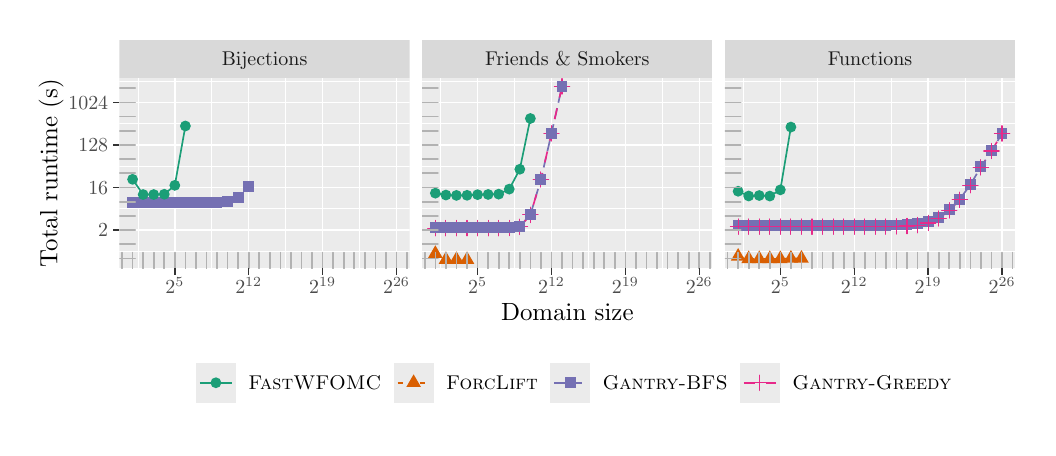
\begin{tikzpicture}[x=1pt,y=1pt]
\definecolor{fillColor}{RGB}{255,255,255}
\path[use as bounding box,fill=fillColor,fill opacity=0.00] (0,0) rectangle (361.35,144.54);
\begin{scope}
\path[clip] (  0.00,  0.00) rectangle (361.35,144.54);
\definecolor{drawColor}{RGB}{255,255,255}
\definecolor{fillColor}{RGB}{255,255,255}

\path[draw=drawColor,line width= 0.5pt,line join=round,line cap=round,fill=fillColor] (  0.00,  0.00) rectangle (361.35,144.54);
\end{scope}
\begin{scope}
\path[clip] ( 33.14, 57.56) rectangle (138.05,126.48);
\definecolor{fillColor}{gray}{0.92}

\path[fill=fillColor] ( 33.14, 57.56) rectangle (138.05,126.48);
\definecolor{drawColor}{RGB}{255,255,255}

\path[draw=drawColor,line width= 0.2pt,line join=round] ( 33.14, 63.71) --
	(138.05, 63.71);

\path[draw=drawColor,line width= 0.2pt,line join=round] ( 33.14, 79.10) --
	(138.05, 79.10);

\path[draw=drawColor,line width= 0.2pt,line join=round] ( 33.14, 94.48) --
	(138.05, 94.48);

\path[draw=drawColor,line width= 0.2pt,line join=round] ( 33.14,109.86) --
	(138.05,109.86);

\path[draw=drawColor,line width= 0.2pt,line join=round] ( 33.14,125.24) --
	(138.05,125.24);

\path[draw=drawColor,line width= 0.2pt,line join=round] ( 39.82, 57.56) --
	( 39.82,126.48);

\path[draw=drawColor,line width= 0.2pt,line join=round] ( 66.52, 57.56) --
	( 66.52,126.48);

\path[draw=drawColor,line width= 0.2pt,line join=round] ( 93.22, 57.56) --
	( 93.22,126.48);

\path[draw=drawColor,line width= 0.2pt,line join=round] (119.93, 57.56) --
	(119.93,126.48);

\path[draw=drawColor,line width= 0.5pt,line join=round] ( 33.14, 71.41) --
	(138.05, 71.41);

\path[draw=drawColor,line width= 0.5pt,line join=round] ( 33.14, 86.79) --
	(138.05, 86.79);

\path[draw=drawColor,line width= 0.5pt,line join=round] ( 33.14,102.17) --
	(138.05,102.17);

\path[draw=drawColor,line width= 0.5pt,line join=round] ( 33.14,117.55) --
	(138.05,117.55);

\path[draw=drawColor,line width= 0.5pt,line join=round] ( 53.17, 57.56) --
	( 53.17,126.48);

\path[draw=drawColor,line width= 0.5pt,line join=round] ( 79.87, 57.56) --
	( 79.87,126.48);

\path[draw=drawColor,line width= 0.5pt,line join=round] (106.58, 57.56) --
	(106.58,126.48);

\path[draw=drawColor,line width= 0.5pt,line join=round] (133.28, 57.56) --
	(133.28,126.48);
\definecolor{drawColor}{RGB}{27,158,119}

\path[draw=drawColor,line width= 0.6pt,line join=round] ( 37.91, 89.74) --
	( 41.73, 84.24) --
	( 45.54, 84.24) --
	( 49.36, 84.34) --
	( 53.17, 87.56) --
	( 56.99,109.01);
\definecolor{drawColor}{RGB}{117,112,179}

\path[draw=drawColor,line width= 0.6pt,dash pattern=on 4pt off 2pt ,line join=round] ( 37.91, 81.38) --
	( 41.73, 81.38) --
	( 45.54, 81.38) --
	( 49.36, 81.38) --
	( 53.17, 81.38) --
	( 56.99, 81.38) --
	( 60.80, 81.39) --
	( 64.62, 81.41) --
	( 68.43, 81.49) --
	( 72.24, 81.81) --
	( 76.06, 83.15) --
	( 79.87, 87.02);
\definecolor{fillColor}{RGB}{117,112,179}

\path[fill=fillColor] ( 35.95, 79.42) --
	( 39.87, 79.42) --
	( 39.87, 83.35) --
	( 35.95, 83.35) --
	cycle;

\path[fill=fillColor] ( 39.77, 79.42) --
	( 43.69, 79.42) --
	( 43.69, 83.35) --
	( 39.77, 83.35) --
	cycle;

\path[fill=fillColor] ( 43.58, 79.42) --
	( 47.50, 79.42) --
	( 47.50, 83.35) --
	( 43.58, 83.35) --
	cycle;

\path[fill=fillColor] ( 47.39, 79.42) --
	( 51.32, 79.42) --
	( 51.32, 83.35) --
	( 47.39, 83.35) --
	cycle;

\path[fill=fillColor] ( 51.21, 79.42) --
	( 55.13, 79.42) --
	( 55.13, 83.35) --
	( 51.21, 83.35) --
	cycle;

\path[fill=fillColor] ( 55.02, 79.42) --
	( 58.95, 79.42) --
	( 58.95, 83.35) --
	( 55.02, 83.35) --
	cycle;

\path[fill=fillColor] ( 58.84, 79.43) --
	( 62.76, 79.43) --
	( 62.76, 83.35) --
	( 58.84, 83.35) --
	cycle;

\path[fill=fillColor] ( 62.65, 79.45) --
	( 66.58, 79.45) --
	( 66.58, 83.37) --
	( 62.65, 83.37) --
	cycle;

\path[fill=fillColor] ( 66.47, 79.53) --
	( 70.39, 79.53) --
	( 70.39, 83.45) --
	( 66.47, 83.45) --
	cycle;

\path[fill=fillColor] ( 70.28, 79.84) --
	( 74.21, 79.84) --
	( 74.21, 83.77) --
	( 70.28, 83.77) --
	cycle;

\path[fill=fillColor] ( 74.10, 81.19) --
	( 78.02, 81.19) --
	( 78.02, 85.11) --
	( 74.10, 85.11) --
	cycle;

\path[fill=fillColor] ( 77.91, 85.05) --
	( 81.84, 85.05) --
	( 81.84, 88.98) --
	( 77.91, 88.98) --
	cycle;
\definecolor{fillColor}{RGB}{27,158,119}

\path[fill=fillColor] ( 37.91, 89.74) circle (  1.96);

\path[fill=fillColor] ( 41.73, 84.24) circle (  1.96);

\path[fill=fillColor] ( 45.54, 84.24) circle (  1.96);

\path[fill=fillColor] ( 49.36, 84.34) circle (  1.96);

\path[fill=fillColor] ( 53.17, 87.56) circle (  1.96);

\path[fill=fillColor] ( 56.99,109.01) circle (  1.96);
\definecolor{drawColor}{gray}{0.70}

\path[draw=drawColor,line width= 0.6pt,line join=round,line cap=round] ( 34.10, 57.56) -- ( 34.10, 63.25);

\path[draw=drawColor,line width= 0.6pt,line join=round,line cap=round] ( 37.91, 57.56) -- ( 37.91, 63.25);

\path[draw=drawColor,line width= 0.6pt,line join=round,line cap=round] ( 41.73, 57.56) -- ( 41.73, 63.25);

\path[draw=drawColor,line width= 0.6pt,line join=round,line cap=round] ( 45.54, 57.56) -- ( 45.54, 63.25);

\path[draw=drawColor,line width= 0.6pt,line join=round,line cap=round] ( 49.36, 57.56) -- ( 49.36, 63.25);

\path[draw=drawColor,line width= 0.6pt,line join=round,line cap=round] ( 53.17, 57.56) -- ( 53.17, 63.25);

\path[draw=drawColor,line width= 0.6pt,line join=round,line cap=round] ( 56.99, 57.56) -- ( 56.99, 63.25);

\path[draw=drawColor,line width= 0.6pt,line join=round,line cap=round] ( 60.80, 57.56) -- ( 60.80, 63.25);

\path[draw=drawColor,line width= 0.6pt,line join=round,line cap=round] ( 64.62, 57.56) -- ( 64.62, 63.25);

\path[draw=drawColor,line width= 0.6pt,line join=round,line cap=round] ( 68.43, 57.56) -- ( 68.43, 63.25);

\path[draw=drawColor,line width= 0.6pt,line join=round,line cap=round] ( 72.24, 57.56) -- ( 72.24, 63.25);

\path[draw=drawColor,line width= 0.6pt,line join=round,line cap=round] ( 76.06, 57.56) -- ( 76.06, 63.25);

\path[draw=drawColor,line width= 0.6pt,line join=round,line cap=round] ( 79.87, 57.56) -- ( 79.87, 63.25);

\path[draw=drawColor,line width= 0.6pt,line join=round,line cap=round] ( 83.69, 57.56) -- ( 83.69, 63.25);

\path[draw=drawColor,line width= 0.6pt,line join=round,line cap=round] ( 87.50, 57.56) -- ( 87.50, 63.25);

\path[draw=drawColor,line width= 0.6pt,line join=round,line cap=round] ( 91.32, 57.56) -- ( 91.32, 63.25);

\path[draw=drawColor,line width= 0.6pt,line join=round,line cap=round] ( 95.13, 57.56) -- ( 95.13, 63.25);

\path[draw=drawColor,line width= 0.6pt,line join=round,line cap=round] ( 98.95, 57.56) -- ( 98.95, 63.25);

\path[draw=drawColor,line width= 0.6pt,line join=round,line cap=round] (102.76, 57.56) -- (102.76, 63.25);

\path[draw=drawColor,line width= 0.6pt,line join=round,line cap=round] (106.58, 57.56) -- (106.58, 63.25);

\path[draw=drawColor,line width= 0.6pt,line join=round,line cap=round] (110.39, 57.56) -- (110.39, 63.25);

\path[draw=drawColor,line width= 0.6pt,line join=round,line cap=round] (114.21, 57.56) -- (114.21, 63.25);

\path[draw=drawColor,line width= 0.6pt,line join=round,line cap=round] (118.02, 57.56) -- (118.02, 63.25);

\path[draw=drawColor,line width= 0.6pt,line join=round,line cap=round] (121.83, 57.56) -- (121.83, 63.25);

\path[draw=drawColor,line width= 0.6pt,line join=round,line cap=round] (125.65, 57.56) -- (125.65, 63.25);

\path[draw=drawColor,line width= 0.6pt,line join=round,line cap=round] (129.46, 57.56) -- (129.46, 63.25);

\path[draw=drawColor,line width= 0.6pt,line join=round,line cap=round] (133.28, 57.56) -- (133.28, 63.25);

\path[draw=drawColor,line width= 0.6pt,line join=round,line cap=round] (137.09, 57.56) -- (137.09, 63.25);

\path[draw=drawColor,line width= 0.6pt,line join=round,line cap=round] ( 33.14, 61.15) -- ( 38.84, 61.15);

\path[draw=drawColor,line width= 0.6pt,line join=round,line cap=round] ( 33.14, 66.28) -- ( 38.84, 66.28);

\path[draw=drawColor,line width= 0.6pt,line join=round,line cap=round] ( 33.14, 71.41) -- ( 38.84, 71.41);

\path[draw=drawColor,line width= 0.6pt,line join=round,line cap=round] ( 33.14, 76.53) -- ( 38.84, 76.53);

\path[draw=drawColor,line width= 0.6pt,line join=round,line cap=round] ( 33.14, 81.66) -- ( 38.84, 81.66);

\path[draw=drawColor,line width= 0.6pt,line join=round,line cap=round] ( 33.14, 86.79) -- ( 38.84, 86.79);

\path[draw=drawColor,line width= 0.6pt,line join=round,line cap=round] ( 33.14, 91.91) -- ( 38.84, 91.91);

\path[draw=drawColor,line width= 0.6pt,line join=round,line cap=round] ( 33.14, 97.04) -- ( 38.84, 97.04);

\path[draw=drawColor,line width= 0.6pt,line join=round,line cap=round] ( 33.14,102.17) -- ( 38.84,102.17);

\path[draw=drawColor,line width= 0.6pt,line join=round,line cap=round] ( 33.14,107.30) -- ( 38.84,107.30);

\path[draw=drawColor,line width= 0.6pt,line join=round,line cap=round] ( 33.14,112.42) -- ( 38.84,112.42);

\path[draw=drawColor,line width= 0.6pt,line join=round,line cap=round] ( 33.14,117.55) -- ( 38.84,117.55);

\path[draw=drawColor,line width= 0.6pt,line join=round,line cap=round] ( 33.14,122.68) -- ( 38.84,122.68);
\end{scope}
\begin{scope}
\path[clip] (142.55, 57.56) rectangle (247.45,126.48);
\definecolor{fillColor}{gray}{0.92}

\path[fill=fillColor] (142.55, 57.56) rectangle (247.45,126.48);
\definecolor{drawColor}{RGB}{255,255,255}

\path[draw=drawColor,line width= 0.2pt,line join=round] (142.55, 63.71) --
	(247.45, 63.71);

\path[draw=drawColor,line width= 0.2pt,line join=round] (142.55, 79.10) --
	(247.45, 79.10);

\path[draw=drawColor,line width= 0.2pt,line join=round] (142.55, 94.48) --
	(247.45, 94.48);

\path[draw=drawColor,line width= 0.2pt,line join=round] (142.55,109.86) --
	(247.45,109.86);

\path[draw=drawColor,line width= 0.2pt,line join=round] (142.55,125.24) --
	(247.45,125.24);

\path[draw=drawColor,line width= 0.2pt,line join=round] (149.22, 57.56) --
	(149.22,126.48);

\path[draw=drawColor,line width= 0.2pt,line join=round] (175.92, 57.56) --
	(175.92,126.48);

\path[draw=drawColor,line width= 0.2pt,line join=round] (202.63, 57.56) --
	(202.63,126.48);

\path[draw=drawColor,line width= 0.2pt,line join=round] (229.33, 57.56) --
	(229.33,126.48);

\path[draw=drawColor,line width= 0.5pt,line join=round] (142.55, 71.41) --
	(247.45, 71.41);

\path[draw=drawColor,line width= 0.5pt,line join=round] (142.55, 86.79) --
	(247.45, 86.79);

\path[draw=drawColor,line width= 0.5pt,line join=round] (142.55,102.17) --
	(247.45,102.17);

\path[draw=drawColor,line width= 0.5pt,line join=round] (142.55,117.55) --
	(247.45,117.55);

\path[draw=drawColor,line width= 0.5pt,line join=round] (162.57, 57.56) --
	(162.57,126.48);

\path[draw=drawColor,line width= 0.5pt,line join=round] (189.28, 57.56) --
	(189.28,126.48);

\path[draw=drawColor,line width= 0.5pt,line join=round] (215.98, 57.56) --
	(215.98,126.48);

\path[draw=drawColor,line width= 0.5pt,line join=round] (242.68, 57.56) --
	(242.68,126.48);
\definecolor{drawColor}{RGB}{27,158,119}

\path[draw=drawColor,line width= 0.6pt,line join=round] (147.31, 84.74) --
	(151.13, 84.06) --
	(154.94, 83.93) --
	(158.76, 83.97) --
	(162.57, 84.20) --
	(166.39, 84.27) --
	(170.20, 84.38) --
	(174.02, 86.20) --
	(177.83, 93.38) --
	(181.65,111.72);
\definecolor{drawColor}{RGB}{217,95,2}

\path[draw=drawColor,line width= 0.6pt,dash pattern=on 2pt off 2pt ,line join=round] (147.31, 62.86) --
	(151.13, 60.69) --
	(154.94, 60.69) --
	(158.76, 60.69);
\definecolor{drawColor}{RGB}{117,112,179}

\path[draw=drawColor,line width= 0.6pt,dash pattern=on 4pt off 2pt ,line join=round] (147.31, 72.23) --
	(151.13, 72.23) --
	(154.94, 72.23) --
	(158.76, 72.23) --
	(162.57, 72.23) --
	(166.39, 72.23) --
	(170.20, 72.23) --
	(174.02, 72.27) --
	(177.83, 72.70) --
	(181.65, 76.95) --
	(185.46, 89.66) --
	(189.28,106.37) --
	(193.09,123.35);
\definecolor{drawColor}{RGB}{231,41,138}

\path[draw=drawColor,line width= 0.6pt,dash pattern=on 4pt off 4pt ,line join=round] (147.31, 72.11) --
	(151.13, 72.11) --
	(154.94, 72.11) --
	(158.76, 72.11) --
	(162.57, 72.11) --
	(166.39, 72.11) --
	(170.20, 72.11) --
	(174.02, 72.15) --
	(177.83, 72.59) --
	(181.65, 76.89) --
	(185.46, 89.67) --
	(189.28,106.37) --
	(193.09,123.35);
\definecolor{fillColor}{RGB}{27,158,119}

\path[fill=fillColor] (147.31, 84.74) circle (  1.96);

\path[fill=fillColor] (151.13, 84.06) circle (  1.96);

\path[fill=fillColor] (154.94, 83.93) circle (  1.96);

\path[fill=fillColor] (158.76, 83.97) circle (  1.96);

\path[fill=fillColor] (162.57, 84.20) circle (  1.96);

\path[fill=fillColor] (166.39, 84.27) circle (  1.96);

\path[fill=fillColor] (170.20, 84.38) circle (  1.96);

\path[fill=fillColor] (174.02, 86.20) circle (  1.96);

\path[fill=fillColor] (177.83, 93.38) circle (  1.96);

\path[fill=fillColor] (181.65,111.72) circle (  1.96);

\path[draw=drawColor,line width= 0.4pt,line join=round,line cap=round] (144.54, 72.11) -- (150.09, 72.11);

\path[draw=drawColor,line width= 0.4pt,line join=round,line cap=round] (147.31, 69.34) -- (147.31, 74.89);

\path[draw=drawColor,line width= 0.4pt,line join=round,line cap=round] (148.35, 72.11) -- (153.90, 72.11);

\path[draw=drawColor,line width= 0.4pt,line join=round,line cap=round] (151.13, 69.33) -- (151.13, 74.88);

\path[draw=drawColor,line width= 0.4pt,line join=round,line cap=round] (152.17, 72.11) -- (157.72, 72.11);

\path[draw=drawColor,line width= 0.4pt,line join=round,line cap=round] (154.94, 69.33) -- (154.94, 74.88);

\path[draw=drawColor,line width= 0.4pt,line join=round,line cap=round] (155.98, 72.11) -- (161.53, 72.11);

\path[draw=drawColor,line width= 0.4pt,line join=round,line cap=round] (158.76, 69.33) -- (158.76, 74.88);

\path[draw=drawColor,line width= 0.4pt,line join=round,line cap=round] (159.80, 72.11) -- (165.35, 72.11);

\path[draw=drawColor,line width= 0.4pt,line join=round,line cap=round] (162.57, 69.33) -- (162.57, 74.88);

\path[draw=drawColor,line width= 0.4pt,line join=round,line cap=round] (163.61, 72.11) -- (169.16, 72.11);

\path[draw=drawColor,line width= 0.4pt,line join=round,line cap=round] (166.39, 69.33) -- (166.39, 74.88);

\path[draw=drawColor,line width= 0.4pt,line join=round,line cap=round] (167.43, 72.11) -- (172.98, 72.11);

\path[draw=drawColor,line width= 0.4pt,line join=round,line cap=round] (170.20, 69.34) -- (170.20, 74.89);

\path[draw=drawColor,line width= 0.4pt,line join=round,line cap=round] (171.24, 72.15) -- (176.79, 72.15);

\path[draw=drawColor,line width= 0.4pt,line join=round,line cap=round] (174.02, 69.37) -- (174.02, 74.92);

\path[draw=drawColor,line width= 0.4pt,line join=round,line cap=round] (175.06, 72.59) -- (180.61, 72.59);

\path[draw=drawColor,line width= 0.4pt,line join=round,line cap=round] (177.83, 69.81) -- (177.83, 75.36);

\path[draw=drawColor,line width= 0.4pt,line join=round,line cap=round] (178.87, 76.89) -- (184.42, 76.89);

\path[draw=drawColor,line width= 0.4pt,line join=round,line cap=round] (181.65, 74.12) -- (181.65, 79.67);

\path[draw=drawColor,line width= 0.4pt,line join=round,line cap=round] (182.69, 89.67) -- (188.24, 89.67);

\path[draw=drawColor,line width= 0.4pt,line join=round,line cap=round] (185.46, 86.90) -- (185.46, 92.45);

\path[draw=drawColor,line width= 0.4pt,line join=round,line cap=round] (186.50,106.37) -- (192.05,106.37);

\path[draw=drawColor,line width= 0.4pt,line join=round,line cap=round] (189.28,103.59) -- (189.28,109.14);

\path[draw=drawColor,line width= 0.4pt,line join=round,line cap=round] (190.32,123.35) -- (195.86,123.35);

\path[draw=drawColor,line width= 0.4pt,line join=round,line cap=round] (193.09,120.57) -- (193.09,126.12);
\definecolor{fillColor}{RGB}{217,95,2}

\path[fill=fillColor] (147.31, 65.91) --
	(149.96, 61.33) --
	(144.67, 61.33) --
	cycle;

\path[fill=fillColor] (151.13, 63.74) --
	(153.77, 59.17) --
	(148.49, 59.17) --
	cycle;

\path[fill=fillColor] (154.94, 63.74) --
	(157.59, 59.17) --
	(152.30, 59.17) --
	cycle;

\path[fill=fillColor] (158.76, 63.74) --
	(161.40, 59.17) --
	(156.12, 59.17) --
	cycle;
\definecolor{fillColor}{RGB}{117,112,179}

\path[fill=fillColor] (145.35, 70.27) --
	(149.28, 70.27) --
	(149.28, 74.20) --
	(145.35, 74.20) --
	cycle;

\path[fill=fillColor] (149.17, 70.27) --
	(153.09, 70.27) --
	(153.09, 74.19) --
	(149.17, 74.19) --
	cycle;

\path[fill=fillColor] (152.98, 70.27) --
	(156.91, 70.27) --
	(156.91, 74.19) --
	(152.98, 74.19) --
	cycle;

\path[fill=fillColor] (156.80, 70.27) --
	(160.72, 70.27) --
	(160.72, 74.19) --
	(156.80, 74.19) --
	cycle;

\path[fill=fillColor] (160.61, 70.27) --
	(164.54, 70.27) --
	(164.54, 74.19) --
	(160.61, 74.19) --
	cycle;

\path[fill=fillColor] (164.43, 70.27) --
	(168.35, 70.27) --
	(168.35, 74.19) --
	(164.43, 74.19) --
	cycle;

\path[fill=fillColor] (168.24, 70.27) --
	(172.16, 70.27) --
	(172.16, 74.20) --
	(168.24, 74.20) --
	cycle;

\path[fill=fillColor] (172.05, 70.31) --
	(175.98, 70.31) --
	(175.98, 74.23) --
	(172.05, 74.23) --
	cycle;

\path[fill=fillColor] (175.87, 70.74) --
	(179.79, 70.74) --
	(179.79, 74.66) --
	(175.87, 74.66) --
	cycle;

\path[fill=fillColor] (179.68, 74.99) --
	(183.61, 74.99) --
	(183.61, 78.91) --
	(179.68, 78.91) --
	cycle;

\path[fill=fillColor] (183.50, 87.70) --
	(187.42, 87.70) --
	(187.42, 91.62) --
	(183.50, 91.62) --
	cycle;

\path[fill=fillColor] (187.31,104.41) --
	(191.24,104.41) --
	(191.24,108.33) --
	(187.31,108.33) --
	cycle;

\path[fill=fillColor] (191.13,121.39) --
	(195.05,121.39) --
	(195.05,125.31) --
	(191.13,125.31) --
	cycle;
\definecolor{drawColor}{gray}{0.70}

\path[draw=drawColor,line width= 0.6pt,line join=round,line cap=round] (143.50, 57.56) -- (143.50, 63.25);

\path[draw=drawColor,line width= 0.6pt,line join=round,line cap=round] (147.31, 57.56) -- (147.31, 63.25);

\path[draw=drawColor,line width= 0.6pt,line join=round,line cap=round] (151.13, 57.56) -- (151.13, 63.25);

\path[draw=drawColor,line width= 0.6pt,line join=round,line cap=round] (154.94, 57.56) -- (154.94, 63.25);

\path[draw=drawColor,line width= 0.6pt,line join=round,line cap=round] (158.76, 57.56) -- (158.76, 63.25);

\path[draw=drawColor,line width= 0.6pt,line join=round,line cap=round] (162.57, 57.56) -- (162.57, 63.25);

\path[draw=drawColor,line width= 0.6pt,line join=round,line cap=round] (166.39, 57.56) -- (166.39, 63.25);

\path[draw=drawColor,line width= 0.6pt,line join=round,line cap=round] (170.20, 57.56) -- (170.20, 63.25);

\path[draw=drawColor,line width= 0.6pt,line join=round,line cap=round] (174.02, 57.56) -- (174.02, 63.25);

\path[draw=drawColor,line width= 0.6pt,line join=round,line cap=round] (177.83, 57.56) -- (177.83, 63.25);

\path[draw=drawColor,line width= 0.6pt,line join=round,line cap=round] (181.65, 57.56) -- (181.65, 63.25);

\path[draw=drawColor,line width= 0.6pt,line join=round,line cap=round] (185.46, 57.56) -- (185.46, 63.25);

\path[draw=drawColor,line width= 0.6pt,line join=round,line cap=round] (189.28, 57.56) -- (189.28, 63.25);

\path[draw=drawColor,line width= 0.6pt,line join=round,line cap=round] (193.09, 57.56) -- (193.09, 63.25);

\path[draw=drawColor,line width= 0.6pt,line join=round,line cap=round] (196.90, 57.56) -- (196.90, 63.25);

\path[draw=drawColor,line width= 0.6pt,line join=round,line cap=round] (200.72, 57.56) -- (200.72, 63.25);

\path[draw=drawColor,line width= 0.6pt,line join=round,line cap=round] (204.53, 57.56) -- (204.53, 63.25);

\path[draw=drawColor,line width= 0.6pt,line join=round,line cap=round] (208.35, 57.56) -- (208.35, 63.25);

\path[draw=drawColor,line width= 0.6pt,line join=round,line cap=round] (212.16, 57.56) -- (212.16, 63.25);

\path[draw=drawColor,line width= 0.6pt,line join=round,line cap=round] (215.98, 57.56) -- (215.98, 63.25);

\path[draw=drawColor,line width= 0.6pt,line join=round,line cap=round] (219.79, 57.56) -- (219.79, 63.25);

\path[draw=drawColor,line width= 0.6pt,line join=round,line cap=round] (223.61, 57.56) -- (223.61, 63.25);

\path[draw=drawColor,line width= 0.6pt,line join=round,line cap=round] (227.42, 57.56) -- (227.42, 63.25);

\path[draw=drawColor,line width= 0.6pt,line join=round,line cap=round] (231.24, 57.56) -- (231.24, 63.25);

\path[draw=drawColor,line width= 0.6pt,line join=round,line cap=round] (235.05, 57.56) -- (235.05, 63.25);

\path[draw=drawColor,line width= 0.6pt,line join=round,line cap=round] (238.87, 57.56) -- (238.87, 63.25);

\path[draw=drawColor,line width= 0.6pt,line join=round,line cap=round] (242.68, 57.56) -- (242.68, 63.25);

\path[draw=drawColor,line width= 0.6pt,line join=round,line cap=round] (246.49, 57.56) -- (246.49, 63.25);

\path[draw=drawColor,line width= 0.6pt,line join=round,line cap=round] (142.55, 61.15) -- (148.24, 61.15);

\path[draw=drawColor,line width= 0.6pt,line join=round,line cap=round] (142.55, 66.28) -- (148.24, 66.28);

\path[draw=drawColor,line width= 0.6pt,line join=round,line cap=round] (142.55, 71.41) -- (148.24, 71.41);

\path[draw=drawColor,line width= 0.6pt,line join=round,line cap=round] (142.55, 76.53) -- (148.24, 76.53);

\path[draw=drawColor,line width= 0.6pt,line join=round,line cap=round] (142.55, 81.66) -- (148.24, 81.66);

\path[draw=drawColor,line width= 0.6pt,line join=round,line cap=round] (142.55, 86.79) -- (148.24, 86.79);

\path[draw=drawColor,line width= 0.6pt,line join=round,line cap=round] (142.55, 91.91) -- (148.24, 91.91);

\path[draw=drawColor,line width= 0.6pt,line join=round,line cap=round] (142.55, 97.04) -- (148.24, 97.04);

\path[draw=drawColor,line width= 0.6pt,line join=round,line cap=round] (142.55,102.17) -- (148.24,102.17);

\path[draw=drawColor,line width= 0.6pt,line join=round,line cap=round] (142.55,107.30) -- (148.24,107.30);

\path[draw=drawColor,line width= 0.6pt,line join=round,line cap=round] (142.55,112.42) -- (148.24,112.42);

\path[draw=drawColor,line width= 0.6pt,line join=round,line cap=round] (142.55,117.55) -- (148.24,117.55);

\path[draw=drawColor,line width= 0.6pt,line join=round,line cap=round] (142.55,122.68) -- (148.24,122.68);
\end{scope}
\begin{scope}
\path[clip] (251.95, 57.56) rectangle (356.85,126.48);
\definecolor{fillColor}{gray}{0.92}

\path[fill=fillColor] (251.95, 57.56) rectangle (356.85,126.48);
\definecolor{drawColor}{RGB}{255,255,255}

\path[draw=drawColor,line width= 0.2pt,line join=round] (251.95, 63.71) --
	(356.85, 63.71);

\path[draw=drawColor,line width= 0.2pt,line join=round] (251.95, 79.10) --
	(356.85, 79.10);

\path[draw=drawColor,line width= 0.2pt,line join=round] (251.95, 94.48) --
	(356.85, 94.48);

\path[draw=drawColor,line width= 0.2pt,line join=round] (251.95,109.86) --
	(356.85,109.86);

\path[draw=drawColor,line width= 0.2pt,line join=round] (251.95,125.24) --
	(356.85,125.24);

\path[draw=drawColor,line width= 0.2pt,line join=round] (258.62, 57.56) --
	(258.62,126.48);

\path[draw=drawColor,line width= 0.2pt,line join=round] (285.33, 57.56) --
	(285.33,126.48);

\path[draw=drawColor,line width= 0.2pt,line join=round] (312.03, 57.56) --
	(312.03,126.48);

\path[draw=drawColor,line width= 0.2pt,line join=round] (338.73, 57.56) --
	(338.73,126.48);

\path[draw=drawColor,line width= 0.5pt,line join=round] (251.95, 71.41) --
	(356.85, 71.41);

\path[draw=drawColor,line width= 0.5pt,line join=round] (251.95, 86.79) --
	(356.85, 86.79);

\path[draw=drawColor,line width= 0.5pt,line join=round] (251.95,102.17) --
	(356.85,102.17);

\path[draw=drawColor,line width= 0.5pt,line join=round] (251.95,117.55) --
	(356.85,117.55);

\path[draw=drawColor,line width= 0.5pt,line join=round] (271.97, 57.56) --
	(271.97,126.48);

\path[draw=drawColor,line width= 0.5pt,line join=round] (298.68, 57.56) --
	(298.68,126.48);

\path[draw=drawColor,line width= 0.5pt,line join=round] (325.38, 57.56) --
	(325.38,126.48);

\path[draw=drawColor,line width= 0.5pt,line join=round] (352.08, 57.56) --
	(352.08,126.48);
\definecolor{drawColor}{RGB}{27,158,119}

\path[draw=drawColor,line width= 0.6pt,line join=round] (256.72, 85.43) --
	(260.53, 83.72) --
	(264.35, 83.89) --
	(268.16, 83.69) --
	(271.97, 85.93) --
	(275.79,108.62);
\definecolor{drawColor}{RGB}{217,95,2}

\path[draw=drawColor,line width= 0.6pt,dash pattern=on 2pt off 2pt ,line join=round] (256.72, 61.86) --
	(260.53, 61.00) --
	(264.35, 61.00) --
	(268.16, 61.00) --
	(271.97, 61.00) --
	(275.79, 61.15) --
	(279.60, 61.15);
\definecolor{drawColor}{RGB}{117,112,179}

\path[draw=drawColor,line width= 0.6pt,dash pattern=on 4pt off 2pt ,line join=round] (256.72, 73.16) --
	(260.53, 73.16) --
	(264.35, 73.16) --
	(268.16, 73.16) --
	(271.97, 73.16) --
	(275.79, 73.16) --
	(279.60, 73.16) --
	(283.42, 73.16) --
	(287.23, 73.16) --
	(291.05, 73.16) --
	(294.86, 73.16) --
	(298.68, 73.16) --
	(302.49, 73.17) --
	(306.31, 73.17) --
	(310.12, 73.20) --
	(313.94, 73.25) --
	(317.75, 73.38) --
	(321.56, 73.71) --
	(325.38, 74.42) --
	(329.19, 76.07) --
	(333.01, 78.80) --
	(336.82, 82.57) --
	(340.64, 87.78) --
	(344.45, 94.24) --
	(348.27,100.04) --
	(352.08,106.25);
\definecolor{drawColor}{RGB}{231,41,138}

\path[draw=drawColor,line width= 0.6pt,dash pattern=on 4pt off 4pt ,line join=round] (256.72, 72.63) --
	(260.53, 72.63) --
	(264.35, 72.63) --
	(268.16, 72.63) --
	(271.97, 72.63) --
	(275.79, 72.63) --
	(279.60, 72.63) --
	(283.42, 72.63) --
	(287.23, 72.63) --
	(291.05, 72.63) --
	(294.86, 72.63) --
	(298.68, 72.63) --
	(302.49, 72.64) --
	(306.31, 72.64) --
	(310.12, 72.67) --
	(313.94, 72.73) --
	(317.75, 72.87) --
	(321.56, 73.21) --
	(325.38, 73.96) --
	(329.19, 75.58) --
	(333.01, 78.49) --
	(336.82, 82.32) --
	(340.64, 87.62) --
	(344.45, 94.08) --
	(348.27, 99.98) --
	(352.08,106.31);
\definecolor{fillColor}{RGB}{117,112,179}

\path[fill=fillColor] (254.75, 71.20) --
	(258.68, 71.20) --
	(258.68, 75.12) --
	(254.75, 75.12) --
	cycle;

\path[fill=fillColor] (258.57, 71.20) --
	(262.49, 71.20) --
	(262.49, 75.12) --
	(258.57, 75.12) --
	cycle;

\path[fill=fillColor] (262.38, 71.20) --
	(266.31, 71.20) --
	(266.31, 75.12) --
	(262.38, 75.12) --
	cycle;

\path[fill=fillColor] (266.20, 71.20) --
	(270.12, 71.20) --
	(270.12, 75.12) --
	(266.20, 75.12) --
	cycle;

\path[fill=fillColor] (270.01, 71.20) --
	(273.94, 71.20) --
	(273.94, 75.12) --
	(270.01, 75.12) --
	cycle;

\path[fill=fillColor] (273.83, 71.20) --
	(277.75, 71.20) --
	(277.75, 75.12) --
	(273.83, 75.12) --
	cycle;

\path[fill=fillColor] (277.64, 71.20) --
	(281.57, 71.20) --
	(281.57, 75.12) --
	(277.64, 75.12) --
	cycle;

\path[fill=fillColor] (281.46, 71.20) --
	(285.38, 71.20) --
	(285.38, 75.12) --
	(281.46, 75.12) --
	cycle;

\path[fill=fillColor] (285.27, 71.20) --
	(289.20, 71.20) --
	(289.20, 75.12) --
	(285.27, 75.12) --
	cycle;

\path[fill=fillColor] (289.09, 71.20) --
	(293.01, 71.20) --
	(293.01, 75.12) --
	(289.09, 75.12) --
	cycle;

\path[fill=fillColor] (292.90, 71.20) --
	(296.82, 71.20) --
	(296.82, 75.12) --
	(292.90, 75.12) --
	cycle;

\path[fill=fillColor] (296.72, 71.20) --
	(300.64, 71.20) --
	(300.64, 75.12) --
	(296.72, 75.12) --
	cycle;

\path[fill=fillColor] (300.53, 71.21) --
	(304.45, 71.21) --
	(304.45, 75.13) --
	(300.53, 75.13) --
	cycle;

\path[fill=fillColor] (304.34, 71.21) --
	(308.27, 71.21) --
	(308.27, 75.14) --
	(304.34, 75.14) --
	cycle;

\path[fill=fillColor] (308.16, 71.24) --
	(312.08, 71.24) --
	(312.08, 75.16) --
	(308.16, 75.16) --
	cycle;

\path[fill=fillColor] (311.97, 71.29) --
	(315.90, 71.29) --
	(315.90, 75.22) --
	(311.97, 75.22) --
	cycle;

\path[fill=fillColor] (315.79, 71.42) --
	(319.71, 71.42) --
	(319.71, 75.35) --
	(315.79, 75.35) --
	cycle;

\path[fill=fillColor] (319.60, 71.75) --
	(323.53, 71.75) --
	(323.53, 75.67) --
	(319.60, 75.67) --
	cycle;

\path[fill=fillColor] (323.42, 72.46) --
	(327.34, 72.46) --
	(327.34, 76.39) --
	(323.42, 76.39) --
	cycle;

\path[fill=fillColor] (327.23, 74.10) --
	(331.16, 74.10) --
	(331.16, 78.03) --
	(327.23, 78.03) --
	cycle;

\path[fill=fillColor] (331.05, 76.84) --
	(334.97, 76.84) --
	(334.97, 80.76) --
	(331.05, 80.76) --
	cycle;

\path[fill=fillColor] (334.86, 80.61) --
	(338.79, 80.61) --
	(338.79, 84.53) --
	(334.86, 84.53) --
	cycle;

\path[fill=fillColor] (338.68, 85.82) --
	(342.60, 85.82) --
	(342.60, 89.74) --
	(338.68, 89.74) --
	cycle;

\path[fill=fillColor] (342.49, 92.28) --
	(346.41, 92.28) --
	(346.41, 96.20) --
	(342.49, 96.20) --
	cycle;

\path[fill=fillColor] (346.30, 98.07) --
	(350.23, 98.07) --
	(350.23,102.00) --
	(346.30,102.00) --
	cycle;

\path[fill=fillColor] (350.12,104.29) --
	(354.04,104.29) --
	(354.04,108.21) --
	(350.12,108.21) --
	cycle;
\definecolor{fillColor}{RGB}{217,95,2}

\path[fill=fillColor] (256.72, 64.91) --
	(259.36, 60.33) --
	(254.07, 60.33) --
	cycle;

\path[fill=fillColor] (260.53, 64.05) --
	(263.17, 59.48) --
	(257.89, 59.48) --
	cycle;

\path[fill=fillColor] (264.35, 64.05) --
	(266.99, 59.48) --
	(261.70, 59.48) --
	cycle;

\path[fill=fillColor] (268.16, 64.05) --
	(270.80, 59.48) --
	(265.52, 59.48) --
	cycle;

\path[fill=fillColor] (271.97, 64.05) --
	(274.62, 59.48) --
	(269.33, 59.48) --
	cycle;

\path[fill=fillColor] (275.79, 64.20) --
	(278.43, 59.63) --
	(273.15, 59.63) --
	cycle;

\path[fill=fillColor] (279.60, 64.20) --
	(282.25, 59.63) --
	(276.96, 59.63) --
	cycle;
\definecolor{fillColor}{RGB}{27,158,119}

\path[fill=fillColor] (256.72, 85.43) circle (  1.96);

\path[fill=fillColor] (260.53, 83.72) circle (  1.96);

\path[fill=fillColor] (264.35, 83.89) circle (  1.96);

\path[fill=fillColor] (268.16, 83.69) circle (  1.96);

\path[fill=fillColor] (271.97, 85.93) circle (  1.96);

\path[fill=fillColor] (275.79,108.62) circle (  1.96);

\path[draw=drawColor,line width= 0.4pt,line join=round,line cap=round] (253.94, 72.63) -- (259.49, 72.63);

\path[draw=drawColor,line width= 0.4pt,line join=round,line cap=round] (256.72, 69.85) -- (256.72, 75.40);

\path[draw=drawColor,line width= 0.4pt,line join=round,line cap=round] (257.76, 72.63) -- (263.31, 72.63);

\path[draw=drawColor,line width= 0.4pt,line join=round,line cap=round] (260.53, 69.85) -- (260.53, 75.40);

\path[draw=drawColor,line width= 0.4pt,line join=round,line cap=round] (261.57, 72.63) -- (267.12, 72.63);

\path[draw=drawColor,line width= 0.4pt,line join=round,line cap=round] (264.35, 69.85) -- (264.35, 75.40);

\path[draw=drawColor,line width= 0.4pt,line join=round,line cap=round] (265.39, 72.63) -- (270.94, 72.63);

\path[draw=drawColor,line width= 0.4pt,line join=round,line cap=round] (268.16, 69.85) -- (268.16, 75.40);

\path[draw=drawColor,line width= 0.4pt,line join=round,line cap=round] (269.20, 72.63) -- (274.75, 72.63);

\path[draw=drawColor,line width= 0.4pt,line join=round,line cap=round] (271.97, 69.85) -- (271.97, 75.40);

\path[draw=drawColor,line width= 0.4pt,line join=round,line cap=round] (273.01, 72.63) -- (278.56, 72.63);

\path[draw=drawColor,line width= 0.4pt,line join=round,line cap=round] (275.79, 69.85) -- (275.79, 75.40);

\path[draw=drawColor,line width= 0.4pt,line join=round,line cap=round] (276.83, 72.63) -- (282.38, 72.63);

\path[draw=drawColor,line width= 0.4pt,line join=round,line cap=round] (279.60, 69.86) -- (279.60, 75.40);

\path[draw=drawColor,line width= 0.4pt,line join=round,line cap=round] (280.64, 72.63) -- (286.19, 72.63);

\path[draw=drawColor,line width= 0.4pt,line join=round,line cap=round] (283.42, 69.85) -- (283.42, 75.40);

\path[draw=drawColor,line width= 0.4pt,line join=round,line cap=round] (284.46, 72.63) -- (290.01, 72.63);

\path[draw=drawColor,line width= 0.4pt,line join=round,line cap=round] (287.23, 69.85) -- (287.23, 75.40);

\path[draw=drawColor,line width= 0.4pt,line join=round,line cap=round] (288.27, 72.63) -- (293.82, 72.63);

\path[draw=drawColor,line width= 0.4pt,line join=round,line cap=round] (291.05, 69.86) -- (291.05, 75.40);

\path[draw=drawColor,line width= 0.4pt,line join=round,line cap=round] (292.09, 72.63) -- (297.64, 72.63);

\path[draw=drawColor,line width= 0.4pt,line join=round,line cap=round] (294.86, 69.86) -- (294.86, 75.40);

\path[draw=drawColor,line width= 0.4pt,line join=round,line cap=round] (295.90, 72.63) -- (301.45, 72.63);

\path[draw=drawColor,line width= 0.4pt,line join=round,line cap=round] (298.68, 69.86) -- (298.68, 75.40);

\path[draw=drawColor,line width= 0.4pt,line join=round,line cap=round] (299.72, 72.64) -- (305.27, 72.64);

\path[draw=drawColor,line width= 0.4pt,line join=round,line cap=round] (302.49, 69.86) -- (302.49, 75.41);

\path[draw=drawColor,line width= 0.4pt,line join=round,line cap=round] (303.53, 72.64) -- (309.08, 72.64);

\path[draw=drawColor,line width= 0.4pt,line join=round,line cap=round] (306.31, 69.87) -- (306.31, 75.42);

\path[draw=drawColor,line width= 0.4pt,line join=round,line cap=round] (307.35, 72.67) -- (312.90, 72.67);

\path[draw=drawColor,line width= 0.4pt,line join=round,line cap=round] (310.12, 69.90) -- (310.12, 75.45);

\path[draw=drawColor,line width= 0.4pt,line join=round,line cap=round] (311.16, 72.73) -- (316.71, 72.73);

\path[draw=drawColor,line width= 0.4pt,line join=round,line cap=round] (313.94, 69.95) -- (313.94, 75.50);

\path[draw=drawColor,line width= 0.4pt,line join=round,line cap=round] (314.98, 72.87) -- (320.53, 72.87);

\path[draw=drawColor,line width= 0.4pt,line join=round,line cap=round] (317.75, 70.09) -- (317.75, 75.64);

\path[draw=drawColor,line width= 0.4pt,line join=round,line cap=round] (318.79, 73.21) -- (324.34, 73.21);

\path[draw=drawColor,line width= 0.4pt,line join=round,line cap=round] (321.56, 70.44) -- (321.56, 75.99);

\path[draw=drawColor,line width= 0.4pt,line join=round,line cap=round] (322.60, 73.96) -- (328.15, 73.96);

\path[draw=drawColor,line width= 0.4pt,line join=round,line cap=round] (325.38, 71.19) -- (325.38, 76.74);

\path[draw=drawColor,line width= 0.4pt,line join=round,line cap=round] (326.42, 75.58) -- (331.97, 75.58);

\path[draw=drawColor,line width= 0.4pt,line join=round,line cap=round] (329.19, 72.81) -- (329.19, 78.36);

\path[draw=drawColor,line width= 0.4pt,line join=round,line cap=round] (330.23, 78.49) -- (335.78, 78.49);

\path[draw=drawColor,line width= 0.4pt,line join=round,line cap=round] (333.01, 75.72) -- (333.01, 81.27);

\path[draw=drawColor,line width= 0.4pt,line join=round,line cap=round] (334.05, 82.32) -- (339.60, 82.32);

\path[draw=drawColor,line width= 0.4pt,line join=round,line cap=round] (336.82, 79.55) -- (336.82, 85.10);

\path[draw=drawColor,line width= 0.4pt,line join=round,line cap=round] (337.86, 87.62) -- (343.41, 87.62);

\path[draw=drawColor,line width= 0.4pt,line join=round,line cap=round] (340.64, 84.84) -- (340.64, 90.39);

\path[draw=drawColor,line width= 0.4pt,line join=round,line cap=round] (341.68, 94.08) -- (347.23, 94.08);

\path[draw=drawColor,line width= 0.4pt,line join=round,line cap=round] (344.45, 91.31) -- (344.45, 96.86);

\path[draw=drawColor,line width= 0.4pt,line join=round,line cap=round] (345.49, 99.98) -- (351.04, 99.98);

\path[draw=drawColor,line width= 0.4pt,line join=round,line cap=round] (348.27, 97.20) -- (348.27,102.75);

\path[draw=drawColor,line width= 0.4pt,line join=round,line cap=round] (349.31,106.31) -- (354.86,106.31);

\path[draw=drawColor,line width= 0.4pt,line join=round,line cap=round] (352.08,103.54) -- (352.08,109.09);
\definecolor{drawColor}{gray}{0.70}

\path[draw=drawColor,line width= 0.6pt,line join=round,line cap=round] (252.90, 57.56) -- (252.90, 63.25);

\path[draw=drawColor,line width= 0.6pt,line join=round,line cap=round] (256.72, 57.56) -- (256.72, 63.25);

\path[draw=drawColor,line width= 0.6pt,line join=round,line cap=round] (260.53, 57.56) -- (260.53, 63.25);

\path[draw=drawColor,line width= 0.6pt,line join=round,line cap=round] (264.35, 57.56) -- (264.35, 63.25);

\path[draw=drawColor,line width= 0.6pt,line join=round,line cap=round] (268.16, 57.56) -- (268.16, 63.25);

\path[draw=drawColor,line width= 0.6pt,line join=round,line cap=round] (271.97, 57.56) -- (271.97, 63.25);

\path[draw=drawColor,line width= 0.6pt,line join=round,line cap=round] (275.79, 57.56) -- (275.79, 63.25);

\path[draw=drawColor,line width= 0.6pt,line join=round,line cap=round] (279.60, 57.56) -- (279.60, 63.25);

\path[draw=drawColor,line width= 0.6pt,line join=round,line cap=round] (283.42, 57.56) -- (283.42, 63.25);

\path[draw=drawColor,line width= 0.6pt,line join=round,line cap=round] (287.23, 57.56) -- (287.23, 63.25);

\path[draw=drawColor,line width= 0.6pt,line join=round,line cap=round] (291.05, 57.56) -- (291.05, 63.25);

\path[draw=drawColor,line width= 0.6pt,line join=round,line cap=round] (294.86, 57.56) -- (294.86, 63.25);

\path[draw=drawColor,line width= 0.6pt,line join=round,line cap=round] (298.68, 57.56) -- (298.68, 63.25);

\path[draw=drawColor,line width= 0.6pt,line join=round,line cap=round] (302.49, 57.56) -- (302.49, 63.25);

\path[draw=drawColor,line width= 0.6pt,line join=round,line cap=round] (306.31, 57.56) -- (306.31, 63.25);

\path[draw=drawColor,line width= 0.6pt,line join=round,line cap=round] (310.12, 57.56) -- (310.12, 63.25);

\path[draw=drawColor,line width= 0.6pt,line join=round,line cap=round] (313.94, 57.56) -- (313.94, 63.25);

\path[draw=drawColor,line width= 0.6pt,line join=round,line cap=round] (317.75, 57.56) -- (317.75, 63.25);

\path[draw=drawColor,line width= 0.6pt,line join=round,line cap=round] (321.56, 57.56) -- (321.56, 63.25);

\path[draw=drawColor,line width= 0.6pt,line join=round,line cap=round] (325.38, 57.56) -- (325.38, 63.25);

\path[draw=drawColor,line width= 0.6pt,line join=round,line cap=round] (329.19, 57.56) -- (329.19, 63.25);

\path[draw=drawColor,line width= 0.6pt,line join=round,line cap=round] (333.01, 57.56) -- (333.01, 63.25);

\path[draw=drawColor,line width= 0.6pt,line join=round,line cap=round] (336.82, 57.56) -- (336.82, 63.25);

\path[draw=drawColor,line width= 0.6pt,line join=round,line cap=round] (340.64, 57.56) -- (340.64, 63.25);

\path[draw=drawColor,line width= 0.6pt,line join=round,line cap=round] (344.45, 57.56) -- (344.45, 63.25);

\path[draw=drawColor,line width= 0.6pt,line join=round,line cap=round] (348.27, 57.56) -- (348.27, 63.25);

\path[draw=drawColor,line width= 0.6pt,line join=round,line cap=round] (352.08, 57.56) -- (352.08, 63.25);

\path[draw=drawColor,line width= 0.6pt,line join=round,line cap=round] (355.90, 57.56) -- (355.90, 63.25);

\path[draw=drawColor,line width= 0.6pt,line join=round,line cap=round] (251.95, 61.15) -- (257.64, 61.15);

\path[draw=drawColor,line width= 0.6pt,line join=round,line cap=round] (251.95, 66.28) -- (257.64, 66.28);

\path[draw=drawColor,line width= 0.6pt,line join=round,line cap=round] (251.95, 71.41) -- (257.64, 71.41);

\path[draw=drawColor,line width= 0.6pt,line join=round,line cap=round] (251.95, 76.53) -- (257.64, 76.53);

\path[draw=drawColor,line width= 0.6pt,line join=round,line cap=round] (251.95, 81.66) -- (257.64, 81.66);

\path[draw=drawColor,line width= 0.6pt,line join=round,line cap=round] (251.95, 86.79) -- (257.64, 86.79);

\path[draw=drawColor,line width= 0.6pt,line join=round,line cap=round] (251.95, 91.91) -- (257.64, 91.91);

\path[draw=drawColor,line width= 0.6pt,line join=round,line cap=round] (251.95, 97.04) -- (257.64, 97.04);

\path[draw=drawColor,line width= 0.6pt,line join=round,line cap=round] (251.95,102.17) -- (257.64,102.17);

\path[draw=drawColor,line width= 0.6pt,line join=round,line cap=round] (251.95,107.30) -- (257.64,107.30);

\path[draw=drawColor,line width= 0.6pt,line join=round,line cap=round] (251.95,112.42) -- (257.64,112.42);

\path[draw=drawColor,line width= 0.6pt,line join=round,line cap=round] (251.95,117.55) -- (257.64,117.55);

\path[draw=drawColor,line width= 0.6pt,line join=round,line cap=round] (251.95,122.68) -- (257.64,122.68);
\end{scope}
\begin{scope}
\path[clip] ( 33.14,126.48) rectangle (138.05,140.04);
\definecolor{fillColor}{gray}{0.85}

\path[fill=fillColor] ( 33.14,126.48) rectangle (138.05,140.04);
\definecolor{drawColor}{gray}{0.10}

\node[text=drawColor,anchor=base,inner sep=0pt, outer sep=0pt, scale=  0.72] at ( 85.60,130.78) {Bijections};
\end{scope}
\begin{scope}
\path[clip] (142.55,126.48) rectangle (247.45,140.04);
\definecolor{fillColor}{gray}{0.85}

\path[fill=fillColor] (142.55,126.48) rectangle (247.45,140.04);
\definecolor{drawColor}{gray}{0.10}

\node[text=drawColor,anchor=base,inner sep=0pt, outer sep=0pt, scale=  0.72] at (195.00,130.78) {Friends \& Smokers};
\end{scope}
\begin{scope}
\path[clip] (251.95,126.48) rectangle (356.85,140.04);
\definecolor{fillColor}{gray}{0.85}

\path[fill=fillColor] (251.95,126.48) rectangle (356.85,140.04);
\definecolor{drawColor}{gray}{0.10}

\node[text=drawColor,anchor=base,inner sep=0pt, outer sep=0pt, scale=  0.72] at (304.40,130.78) {Functions};
\end{scope}
\begin{scope}
\path[clip] (  0.00,  0.00) rectangle (361.35,144.54);
\definecolor{drawColor}{gray}{0.20}

\path[draw=drawColor,line width= 0.5pt,line join=round] ( 53.17, 55.31) --
	( 53.17, 57.56);

\path[draw=drawColor,line width= 0.5pt,line join=round] ( 79.87, 55.31) --
	( 79.87, 57.56);

\path[draw=drawColor,line width= 0.5pt,line join=round] (106.58, 55.31) --
	(106.58, 57.56);

\path[draw=drawColor,line width= 0.5pt,line join=round] (133.28, 55.31) --
	(133.28, 57.56);
\end{scope}
\begin{scope}
\path[clip] (  0.00,  0.00) rectangle (361.35,144.54);
\definecolor{drawColor}{gray}{0.30}

\node[text=drawColor,anchor=base,inner sep=0pt, outer sep=0pt, scale=  0.72] at ( 53.17, 48.55) {$2^{5}$};

\node[text=drawColor,anchor=base,inner sep=0pt, outer sep=0pt, scale=  0.72] at ( 79.87, 48.55) {$2^{12}$};

\node[text=drawColor,anchor=base,inner sep=0pt, outer sep=0pt, scale=  0.72] at (106.58, 48.55) {$2^{19}$};

\node[text=drawColor,anchor=base,inner sep=0pt, outer sep=0pt, scale=  0.72] at (133.28, 48.55) {$2^{26}$};
\end{scope}
\begin{scope}
\path[clip] (  0.00,  0.00) rectangle (361.35,144.54);
\definecolor{drawColor}{gray}{0.20}

\path[draw=drawColor,line width= 0.5pt,line join=round] (162.57, 55.31) --
	(162.57, 57.56);

\path[draw=drawColor,line width= 0.5pt,line join=round] (189.28, 55.31) --
	(189.28, 57.56);

\path[draw=drawColor,line width= 0.5pt,line join=round] (215.98, 55.31) --
	(215.98, 57.56);

\path[draw=drawColor,line width= 0.5pt,line join=round] (242.68, 55.31) --
	(242.68, 57.56);
\end{scope}
\begin{scope}
\path[clip] (  0.00,  0.00) rectangle (361.35,144.54);
\definecolor{drawColor}{gray}{0.30}

\node[text=drawColor,anchor=base,inner sep=0pt, outer sep=0pt, scale=  0.72] at (162.57, 48.55) {$2^{5}$};

\node[text=drawColor,anchor=base,inner sep=0pt, outer sep=0pt, scale=  0.72] at (189.28, 48.55) {$2^{12}$};

\node[text=drawColor,anchor=base,inner sep=0pt, outer sep=0pt, scale=  0.72] at (215.98, 48.55) {$2^{19}$};

\node[text=drawColor,anchor=base,inner sep=0pt, outer sep=0pt, scale=  0.72] at (242.68, 48.55) {$2^{26}$};
\end{scope}
\begin{scope}
\path[clip] (  0.00,  0.00) rectangle (361.35,144.54);
\definecolor{drawColor}{gray}{0.20}

\path[draw=drawColor,line width= 0.5pt,line join=round] (271.97, 55.31) --
	(271.97, 57.56);

\path[draw=drawColor,line width= 0.5pt,line join=round] (298.68, 55.31) --
	(298.68, 57.56);

\path[draw=drawColor,line width= 0.5pt,line join=round] (325.38, 55.31) --
	(325.38, 57.56);

\path[draw=drawColor,line width= 0.5pt,line join=round] (352.08, 55.31) --
	(352.08, 57.56);
\end{scope}
\begin{scope}
\path[clip] (  0.00,  0.00) rectangle (361.35,144.54);
\definecolor{drawColor}{gray}{0.30}

\node[text=drawColor,anchor=base,inner sep=0pt, outer sep=0pt, scale=  0.72] at (271.97, 48.55) {$2^{5}$};

\node[text=drawColor,anchor=base,inner sep=0pt, outer sep=0pt, scale=  0.72] at (298.68, 48.55) {$2^{12}$};

\node[text=drawColor,anchor=base,inner sep=0pt, outer sep=0pt, scale=  0.72] at (325.38, 48.55) {$2^{19}$};

\node[text=drawColor,anchor=base,inner sep=0pt, outer sep=0pt, scale=  0.72] at (352.08, 48.55) {$2^{26}$};
\end{scope}
\begin{scope}
\path[clip] (  0.00,  0.00) rectangle (361.35,144.54);
\definecolor{drawColor}{gray}{0.30}

\node[text=drawColor,anchor=base east,inner sep=0pt, outer sep=0pt, scale=  0.72] at ( 29.09, 68.93) {2};

\node[text=drawColor,anchor=base east,inner sep=0pt, outer sep=0pt, scale=  0.72] at ( 29.09, 84.31) {16};

\node[text=drawColor,anchor=base east,inner sep=0pt, outer sep=0pt, scale=  0.72] at ( 29.09, 99.69) {128};

\node[text=drawColor,anchor=base east,inner sep=0pt, outer sep=0pt, scale=  0.72] at ( 29.09,115.07) {1024};
\end{scope}
\begin{scope}
\path[clip] (  0.00,  0.00) rectangle (361.35,144.54);
\definecolor{drawColor}{gray}{0.20}

\path[draw=drawColor,line width= 0.5pt,line join=round] ( 30.89, 71.41) --
	( 33.14, 71.41);

\path[draw=drawColor,line width= 0.5pt,line join=round] ( 30.89, 86.79) --
	( 33.14, 86.79);

\path[draw=drawColor,line width= 0.5pt,line join=round] ( 30.89,102.17) --
	( 33.14,102.17);

\path[draw=drawColor,line width= 0.5pt,line join=round] ( 30.89,117.55) --
	( 33.14,117.55);
\end{scope}
\begin{scope}
\path[clip] (  0.00,  0.00) rectangle (361.35,144.54);
\definecolor{drawColor}{RGB}{0,0,0}

\node[text=drawColor,anchor=base,inner sep=0pt, outer sep=0pt, scale=  0.90] at (195.00, 38.70) {Domain size};
\end{scope}
\begin{scope}
\path[clip] (  0.00,  0.00) rectangle (361.35,144.54);
\definecolor{drawColor}{RGB}{0,0,0}

\node[text=drawColor,rotate= 90.00,anchor=base,inner sep=0pt, outer sep=0pt, scale=  0.90] at ( 10.70, 92.02) {Total runtime (s)};
\end{scope}
\begin{scope}
\path[clip] (  0.00,  0.00) rectangle (361.35,144.54);
\definecolor{fillColor}{RGB}{255,255,255}

\path[fill=fillColor] ( 51.80,  4.50) rectangle (338.20, 27.95);
\end{scope}
\begin{scope}
\path[clip] (  0.00,  0.00) rectangle (361.35,144.54);
\definecolor{fillColor}{gray}{0.92}

\path[fill=fillColor] ( 60.80,  9.00) rectangle ( 75.25, 23.45);
\end{scope}
\begin{scope}
\path[clip] (  0.00,  0.00) rectangle (361.35,144.54);
\definecolor{drawColor}{RGB}{27,158,119}

\path[draw=drawColor,line width= 0.6pt,line join=round] ( 62.24, 16.23) -- ( 73.81, 16.23);
\end{scope}
\begin{scope}
\path[clip] (  0.00,  0.00) rectangle (361.35,144.54);
\definecolor{fillColor}{RGB}{27,158,119}

\path[fill=fillColor] ( 68.02, 16.23) circle (  1.96);
\end{scope}
\begin{scope}
\path[clip] (  0.00,  0.00) rectangle (361.35,144.54);
\definecolor{fillColor}{gray}{0.92}

\path[fill=fillColor] (132.24,  9.00) rectangle (146.69, 23.45);
\end{scope}
\begin{scope}
\path[clip] (  0.00,  0.00) rectangle (361.35,144.54);
\definecolor{drawColor}{RGB}{217,95,2}

\path[draw=drawColor,line width= 0.6pt,dash pattern=on 2pt off 2pt ,line join=round] (133.68, 16.23) -- (145.25, 16.23);
\end{scope}
\begin{scope}
\path[clip] (  0.00,  0.00) rectangle (361.35,144.54);
\definecolor{fillColor}{RGB}{217,95,2}

\path[fill=fillColor] (139.46, 19.28) --
	(142.11, 14.70) --
	(136.82, 14.70) --
	cycle;
\end{scope}
\begin{scope}
\path[clip] (  0.00,  0.00) rectangle (361.35,144.54);
\definecolor{fillColor}{gray}{0.92}

\path[fill=fillColor] (188.77,  9.00) rectangle (203.22, 23.45);
\end{scope}
\begin{scope}
\path[clip] (  0.00,  0.00) rectangle (361.35,144.54);
\definecolor{drawColor}{RGB}{117,112,179}

\path[draw=drawColor,line width= 0.6pt,dash pattern=on 4pt off 2pt ,line join=round] (190.22, 16.23) -- (201.78, 16.23);
\end{scope}
\begin{scope}
\path[clip] (  0.00,  0.00) rectangle (361.35,144.54);
\definecolor{fillColor}{RGB}{117,112,179}

\path[fill=fillColor] (194.03, 14.26) --
	(197.96, 14.26) --
	(197.96, 18.19) --
	(194.03, 18.19) --
	cycle;
\end{scope}
\begin{scope}
\path[clip] (  0.00,  0.00) rectangle (361.35,144.54);
\definecolor{fillColor}{gray}{0.92}

\path[fill=fillColor] (257.35,  9.00) rectangle (271.81, 23.45);
\end{scope}
\begin{scope}
\path[clip] (  0.00,  0.00) rectangle (361.35,144.54);
\definecolor{drawColor}{RGB}{231,41,138}

\path[draw=drawColor,line width= 0.6pt,dash pattern=on 4pt off 4pt ,line join=round] (258.80, 16.23) -- (270.36, 16.23);
\end{scope}
\begin{scope}
\path[clip] (  0.00,  0.00) rectangle (361.35,144.54);
\definecolor{drawColor}{RGB}{231,41,138}

\path[draw=drawColor,line width= 0.4pt,line join=round,line cap=round] (261.81, 16.23) -- (267.35, 16.23);

\path[draw=drawColor,line width= 0.4pt,line join=round,line cap=round] (264.58, 13.45) -- (264.58, 19.00);
\end{scope}
\begin{scope}
\path[clip] (  0.00,  0.00) rectangle (361.35,144.54);
\definecolor{drawColor}{RGB}{0,0,0}

\node[text=drawColor,anchor=base west,inner sep=0pt, outer sep=0pt, scale=  0.72] at ( 79.75, 13.75) {\textsc{FastWFOMC}};
\end{scope}
\begin{scope}
\path[clip] (  0.00,  0.00) rectangle (361.35,144.54);
\definecolor{drawColor}{RGB}{0,0,0}

\node[text=drawColor,anchor=base west,inner sep=0pt, outer sep=0pt, scale=  0.72] at (151.19, 13.75) {\textsc{ForcLift}};
\end{scope}
\begin{scope}
\path[clip] (  0.00,  0.00) rectangle (361.35,144.54);
\definecolor{drawColor}{RGB}{0,0,0}

\node[text=drawColor,anchor=base west,inner sep=0pt, outer sep=0pt, scale=  0.72] at (207.72, 13.75) {\textsc{Gantry-BFS}};
\end{scope}
\begin{scope}
\path[clip] (  0.00,  0.00) rectangle (361.35,144.54);
\definecolor{drawColor}{RGB}{0,0,0}

\node[text=drawColor,anchor=base west,inner sep=0pt, outer sep=0pt, scale=  0.72] at (276.31, 13.75) {\textsc{Gantry-Greedy}};
\end{scope}
\end{tikzpicture}

\end{document}

  \caption{The runtime data of WFOMC algorithms on permutation- and
    function-counting problems on domains of sizes $1, 2, \dots, 35$. Note that
    the $y$ axis is on a logarithmic scale.}\label{fig:plot}
\end{figure}

\paragraph{Results.}
\begin{itemize}
  \item As shown in \cref{fig:plot}, the runtimes of all compilation-based
        algorithms remain practically constant in contrast to the rapidly
        increasing runtimes of \textsc{FastWFOMC}.
  \item Note that \Cranebfs{} is able to handle more instances than
        \textsc{ForcLift} (e.g., the permutation-counting problem in our
        experiments and other problems in my previous work).
  \item Although the search/compilation part is slower in \Cranetwo{} than in
        \textsc{ForcLift}, the difference is negligible.
  \item The runtimes of three out of four WFOMC algorithms appear constant
        because---for these counting problems and domain sizes---compilation
        time dominates inference time (recall that compilation time is
        independent of domain sizes). Indeed, the maximum inference time of both
        \Cranebfs{} and \Cranegreedy{} across these experiments is
        only \SI{4}{\milli\second}.
  \item The runtimes of \Cranetwo{} have lower variation than those of
        \textsc{ForcLift} because with \textsc{ForcLift} we compile the formula
        anew for each domain size whereas with \Cranetwo{} we compile it once
        and reuse the resulting C++ program for all domain sizes.
  \item As another point of comparison,---in at most
        \SI{41}{\second}---\Cranetwo{} scales up to domains of sizes \num{e4}
        and \num{3e5} in permutation- and function-counting problems,
        respectively (whereas \textsc{FastWFOMC} already takes longer with
        domains of sizes\dots)
\end{itemize}

\todo[inline]{maybe examine \textsc{ForcLift}'s scalability as well}

\todo[inline,caption={}]{
  Some reproducibility requirements to keep in mind:
  \begin{itemize}
    \item A motivation is given for why the experiments are conducted on the
          selected datasets.
    \item All novel datasets introduced in this paper are included in a data
          appendix.
    \item All datasets drawn from the existing literature (potentially including
          authors’ own previously published work) are accompanied by appropriate
          citations. (mention the counting quantifier paper and my KR paper)
    \item All source code implementing new methods have comments detailing the
          implementation, with references to the paper where each step comes
          from.
    \item This paper formally describes evaluation metrics used and explains the
          motivation for choosing these metrics.
    \item This paper states the number of algorithm runs used to compute each
          reported result.
  \end{itemize}
}

\section{Conclusion (TODO)}

\todo[inline,caption={}]{
  \begin{itemize}
    \item Maybe add some complete examples of C++ programs in the supplementary
          material.
          \item Later on:
          \begin{itemize}
            \item Eliminate (e.g., Emacs) warnings.
            \item must run it by all 3 other coauthors
            \item re-check submission instructions and formatting guidelines
            \item Full stop at the end of a single-sentence caption?
            \item cite the \textsc{Crane} paper (and other algorithms' papers)
                  where necessary
            \item Something to think about that could inspire some kind of
                  theorems: how can I assume that a domain is empty if there are
                  constants associated with it?
          \end{itemize}
  \end{itemize}
}

\clearpage % TODO: temporarary

\bibliographystyle{kr}
\bibliography{paper}

\end{document}
